\documentclass[type=dr, dr=rernat, accentcolor=tud7b,colorbacktitle, bigchapter, openright, twoside, 12pt ]{tudthesis}
%\documentclass[11pt,twoside,a4paper]{article}
\usepackage[english]{babel} 
\usepackage[utf8]{inputenc}
\usepackage{graphicx}
\usepackage{pstricks}
\usepackage{psfrag}
\usepackage{enumerate}
\usepackage{float}
\usepackage{epsfig}
\usepackage{geometry}
\usepackage{subfigure}
\usepackage{rotating}
\usepackage{minitoc}
% \usepackage{dominitoc}
\usepackage{multirow}
%\usepackage{appendix}
%\usepackage[breaklinks=true]{hyperref}
%\usepackage{breakcites}

%%%% 1 1/2 facher Zeilenabstand:	
\usepackage{setspace}
\onehalfspacing




\begin{document}
\chapter{Deformable Image Registration and Validation}
\label{chapter:vmm}
\minitoc

\section{Introduction}

As explained in Section \textbf{ref!}) effects of motion can have a significant impact on a radiation treatment. Therefore a proper investigation is necessary for each specific patient. There are several motion mitigation techniques available that can operate on beam delivery, patient immobilization or treatment planning level.

An important part of motion mitigation is proper and frequent imaging. While most commercial treatment planning software provide rigid registration between different images, deformable image registration (DIR) is currently rarely used. DIR ca quantify anatomical and biological variations better compared to rigid registration \cite{Sarrut2006} and is essential as well in photon as in ion radiotherapy, with usage in adaptive radiotherapy \cite{Yan1997,Yan2010}, 4D optimization \cite{Trofimov2005}, 4D dose calculation \cite{Flampouri2006}, contour propagation \cite{Lu2006b}. DIR usage spreads even into other categories, besides radiotherapy \cite{Cleary2010, Herrell2012, Nithiananthan2011, Naini2010}. Several different DIR algorithms are available, such as B-spline \cite{Rueckert1999}, Deamons \cite{Thirion1998}, linear elastic finite element \cite{Venugopal2005}, optical flow \cite{Zhong2007}, viscous fluid \cite{Christensen1996}, etc.
	
One of the reasons for the DIR is not used in commercial software is the lack of proper DIR quality assurance (DIRQA). While several different DIRQA methods exist, none of them are definitive and most of them are time consuming. It is possible to evaluate DIR with deformable phantoms, where the type and size of deformation is known \cite{Kashani2007, Kirby2011}. However such quality assurance is time consuming and it would be hard to use it in everyday clinical workflow. DIR validation can also be based on landmark positions, specifically their location before and after registration. In absence of externally planted markers, locating landmarks in patient anatomy can be take a fair amount of time and it can be difficult to identify landmarks in low-contrast regions \cite{Varadhan2013}. Another option is to compare delineated contours with the propagated ones. It is more efficient technique than landmark checks, however it is even more time consuming and it does not address the region within the contour.

In this chapter tools to handle motion management, DIR and DIR validation will be presented. Tools were constructed for open-source software 3D Slicer, described in Section~\ref{Slicer}. In Section~\ref{Registration} details on how DIR was performed will be explained. Next, Section~\ref{DIRQA} will address the DIR validation - an extensive tool was created with various features to tackle DIR validation. Section~\ref{Contour} will be about contour visualization. Last two sections in implementation part will be about a tool to display organ motion amplitude and generation of a mid-ventilation CT. Tools were tested on real patient data and results will be presented in the Section~\ref{Verification}. Summary and discussion will be given last to sum up.

\section{Implementation}
\label{Implementation}

\subsection{3D Slicer}
\label{Slicer}

3D Slicer (Slicer) is a software platform for analysis and visualization of medical images \cite{Slicer, Fedorov2012}. Slicer is a free, open-source software (BSD-style license) available on Windows, MacOSX and Linux operating systems. Slicer provides a vast variety of tools, such as:

\begin{itemize}
	\item Handling a variety of image formats, including DICOM, NRRD and MHA
	\item Visualization of voxel images, polygonal meshes and volume renderings
	\item Registration tool (rigid and non-rigid) and display of vector fields
	\item Automatic image segmentation
	\item Analysis and visualization of diffusion tensor image data
	\item Device tracking for image-guided procedures
\end{itemize}

The foundation of Slicer is written in C++ and it's functions can be accessed also with Python to provide rapid, iterative development. Graphical user interface is built in Qt. Visualization is based on VTK, a graphical library commonly used in scientific research.

Slicer is a research tool and as such offers tools to implement new functionalities in the form of 3D Slicer extensions. They can either be as execution of external command-line programs or writing modules with new features or automate Slicer processes in form of scripted modules. 
In the next sections different Slicer modules will be presented, which were all developed in the scope of this thesis. The purpose of modules is to quantify and visualize patient motion as well as to provide quality assurance of the the obtained results.




\subsection{Registration}
\label{Registration}

The changes in patient anatomy can be seen on CT (4DCT) or MRI scan. To assest this changes a registration must be preformed. Registration can be made between different imaging modaleteis, scans from different days or phases in 4DCT. Different algorithms and software is avaliable
for image registration. However, the result is always a transformation map \cite{Richter2012}. 

\begin{equation}
\label{df}
x' = x + u_{ri}(x)
\end{equation} 

Here, $x$ and $x'$ are points in states $r$ and $i$, respectively and $u_{ri}$ is a vector field representation of the transformation map. $u_{ri}$ can among others be used for assesing motion amplitudes, contour propagation and 4D dose reconstruction. It is important to note
that for certain steps in 4D treatment planning require also inverse registration, from state $i$ to $r$ \cite{Richter2012}.

Plastimatch \cite{Shackleford2010} is a comonlly used software for registration in medical research. It is free and open-source software, avaliable as a command-line executable program. Plastimatch B-spline registration is also available in Slicer as an external module, SlicerRT \cite{Pinter2012}.  
The integration of Plastimatch in Slicer brings the advantage of a graphic user interface and hence a quick modification of parameters. However, the disadvantage comes when a large number of registrations is required, since a user presence is required. In a 4DCT registration
there are $2(N-1)$ registrations required - from reference phase to each of $N$ states of 4DCT and vice versa, except for the reference phase itself. Typical 4DCT consist of 10 phases, therefore a automatic registration of a 4DCT is a necessity, since each registration takes from 15-30 minutes.

Rather than just automatically loading different phases and registering them in Slicer a patient hierarchy concept was introduced and is explained in Section~\ref{PatHierarchy}.

\subsubsection{Registration nomenclature}

In order to be able to provide a clear description of methods and procedures used, an overview of the expresions used will be given here.

\begin{itemize}
 \item \textbf{Reference image} - image that serves as a reference position.
 \item \textbf{Moving image} - image that is being registered to the reference image.
 \item \textbf{Warped image} - image resulting from registration. It should be as closed to the image being registered to as possible.
 \item \textbf{True registration} - registration from moving to reference image. Similar, everything connected to true registration will use \"true\" (true vector field, true warped image, true absolute difference, true Jacobian, etc.).
 \item \textbf{Inverse registration} - registration from reference to moving image (oposite or inverse of true registration. As in true registration, term inverse can be used for everything connected to it (inverse vector field, inverse warped image, inverse absolute difference, inverse Jacobian, etc.).
\end{itemize}


\subsubsection{Patient hierarchy} 
\label{PatHierarchy}

Patient hierarchy followes a subject hierarchy principle in Slicer. It was desigened for a clear overview of the registration process, DIRQA and all resulting files. Another reason is to track DIR
and DIRQA in case if they are interupted by Slicer crash. DIR and DIRQA files can be quite large and can cause Slicer to run out of memory. Patient hierarhy enables then to continue work
from where it was interupted.

There are several levels in patient hierarchy. Each level also has different attributes, where details such as file path or reference phase are written.

\begin{itemize}
	\item Level 1: \textbf{Patient name} - seperates different patients.
	\item Level 2: \textbf{Registration node} - seperates between different registration, e.g. registration between 4DCT phases, between CT and 4DCT, MRI and CT... 
	\subitem The file directory of image, vector field and registration quality files is stored as an attribute. Additionally, there are number of phases to be registered and which phase is the reference one.
	\item Level 3: \textbf{Registration phase} - specific registration phase. Registration is done between all phases and the reference one. There have to be at least two phases
	\item Level 4: \textbf{Node} - can be either an image, a vector field, an inverse vector field or any of DIRQA nodes (see Section~\ref{DIRQA}).
	\subitem Exact file paths for specific node is stored as an attribute.
\end{itemize}

Patient hierarchy can be constructed in two ways. First option is to manually crate the whole patient hierarchy, from top to bottom level, with necessary attributes. Second option is using automatic script to look for files on hard drive and create corresponding levels in patient hierarchy. This
is possible only, if some conventions are used regarding file names and locations.

\subsection{Registration Quality Checks}
\label{DIRQA}

In order to provide visual and quantitative assessment of the registration quality a \textbf{Deformable Image Registration Quality Assurance} module was created. It provides different image checks (false color, checkerboard, absolute difference, flicker, movie and landmark positions) and vector checks (Jacobian and inverse consistency error). Details on all different checks will be explained in this section. Reference image, warped image, vector and inverse vector (vector from reference to moving phase) are used as inputs for DIRQA module. Additionaly landmarks and region of interest (ROI) can be used as an input.

All check that use some kind of mathematical operation on or between images (absolute difference, Jacobian and inverse consistency error) were build using tools from ITK library \cite{Yoo2002}.

\subsubsection{False color}
\label{Sec:FalseColor}

A good way to see difference between two images is to overlay them. However, since CT scans are usually displayed in grayscale color code, the differences can become indistinguishable. Especially if the images are quite similar, as reference and warped image usually are. With applying opposite color code to overlaying images two things are achieved. Firstly, regions were the registration was successful will be in grayscale. Furthermore the differences will be in color of image they belong to. In the module we used red and cyan color code for reference and warped image respectively. See Fig.~\ref{falseColor} for details.

\begin{figure}[H]
	\begin{center}		
		
\includegraphics[width=0.9\textwidth]{./Images/falseColor.png}
		\caption{Example of false color overlay. Images (a) and (b) show red and cyan color code, respectively, for CT scan. (c) displays overlayed false colored images before and (d) after registration.}
		\label{falseColor}
	\end{center}
\end{figure}

\subsubsection{Checkerboard}

As the name suggests, checkerboard creates an image of tiles. Each tile alternates between reference and warped image, as shown in Fig.~\ref{checkerboard}. The differences between two images become apparent if there is no smooth transition from one tile to the next. The number of tiles can be manually selected. While the checkerboard offers clear indication of differences, it requires user to spot them - similar to false color.

\begin{figure}[H]
	\begin{center}		
		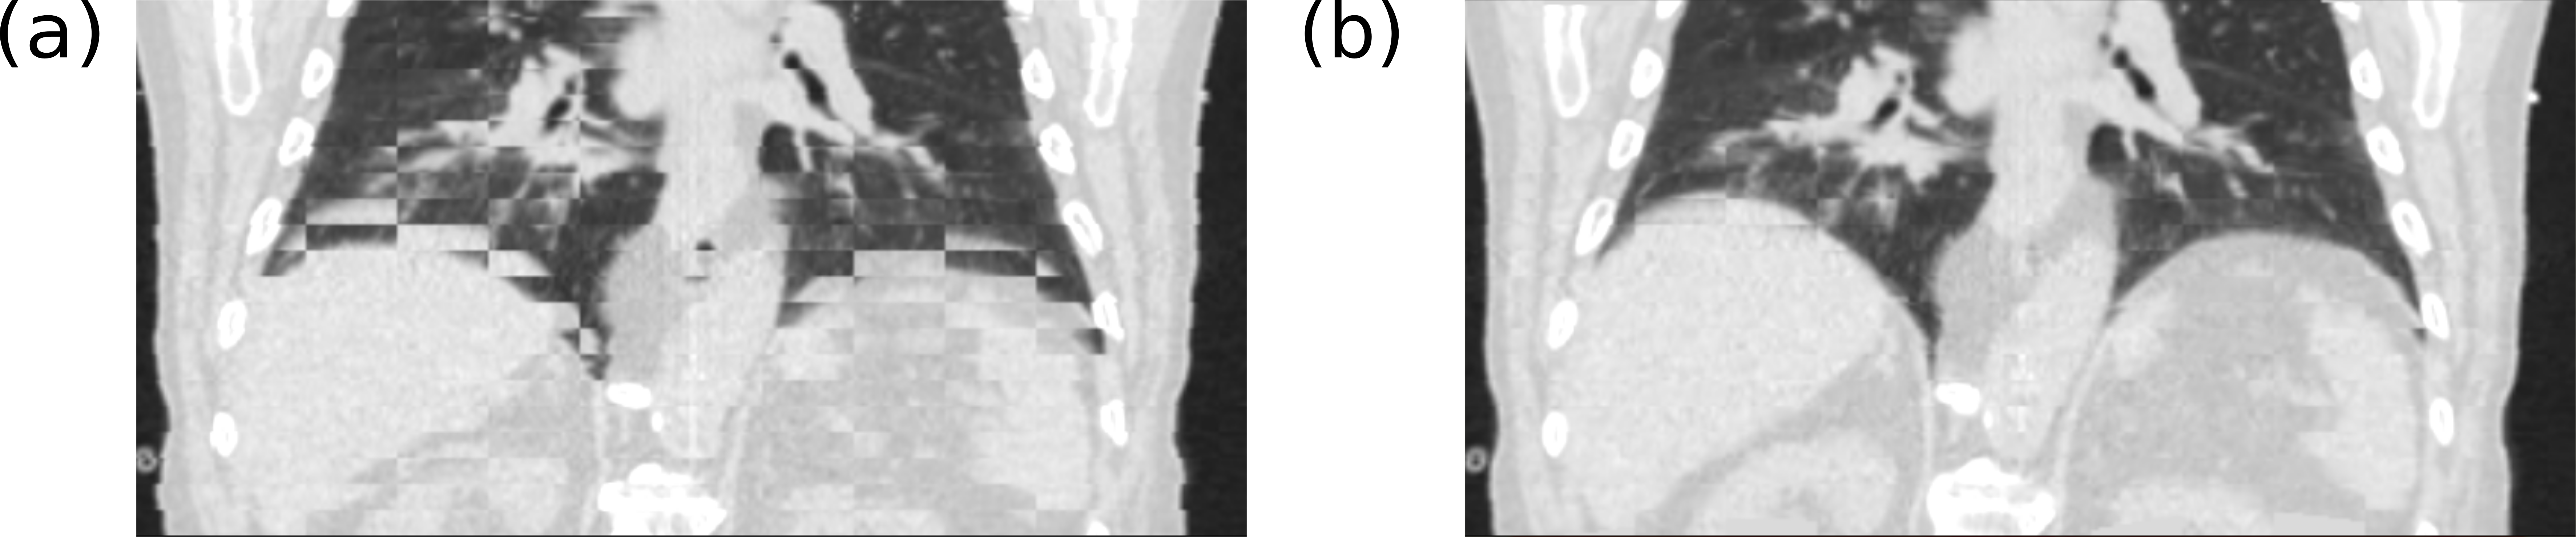
\includegraphics[width=0.9\textwidth]{./Images/checkerboard.png}
		\caption{Example of checkerboard image. Image consist of tiles alternating between two images. Tiles in image (a) alternate between scans before registration and in image (b) after registration.}
		\label{checkerboard}
	\end{center}
\end{figure}

\subsubsection{Absolute difference} 

To stress the difference between reference and warped image an absolute difference between voxel values is calculated and displayed. New image is generated, with voxels populated as the absolute difference between reference and warped image voxel values, as shown in Fig.~\ref{absDiff}. Furthermore, average, standard deviation, minimum and maximum of absolute differneces are calulcated for quantitative assessment of registration quality (in ideal case all values would be 0).

The absolute difference feature is similar to false color, but it displays differences clearer and it also provides quantitative values. In contrast to false color which only relies on user examination. 

Absoulte difference can be computed between reference and moving image, named default absolute difference, to provide initial estimate of difference between images. After the registration it can be done on
true and inverse warped images (true and inverse absolute difference) to show registration results. Usually, registration works on minimizing absolute difference, so it is a direct indicatior
of registration success.

To spare computational time or to focus on a specific region, absolute difference can also be calculated just on a specific ROI (if used as an input). Usually ROI around patient body is selected, rather than calculating on a whole patient CT.


\begin{figure}[H]
	\begin{center}		
		\includegraphics[width=0.9\textwidth]{./Images/abs.png}
		\caption{Absolute difference image before (a) and after registration (b). The mean absolute difference before registration (default absolute difference) is 62 HU and 31 HU after registration (true absolute difference).}
		\label{absDiff}
	\end{center}
\end{figure}

\subsubsection{Movie}

Medical images are usually quite large - typical CT image consist of $512 \times 512 \times 100$ pixels, which makes inspecting image checks (false color, checkerboard, absolute difference) a time-consuming task. Movie feature allows for smoother display of different image slices. User selects, which view he would like to inspect (axial, sagital or coronal) and presses start. Selected views then start scrolling from one limit to the other. It allows user to focus on registration details, rather than scrolling through slices.

Movie and flicker (explained below) do not offer any specific registration check, but improve the process of registration quality assurance.

\subsubsection{Flicker}

While it is possible to display two images side by side in Slicer, it can sometimes be hard to see fine differences between the two images. Flicker alternates between reference and warped image on a single display. Flicker changes image each 0.5 s.

\subsubsection{Landmark positions}

Landmark positions are often used to determine registration spatial accuracy \cite{Castillo2009}. Landmark can either be a specific feature in patient anatomy, or an external marker. The position of the landmark in the warped image would ideally be at the same position as in reference image. The module measures the Euclidean norm between the landmark position in reference and warped image.

User has to manually select landmarks in reference and moving image. For landmarks based on patient anatomy a physician is required. Landmark from moving image can then be automatically transformed with transformation vector field to obtain position in warped image or it can be manually selected in warped image.

\begin{figure}[H]
\begin{center}
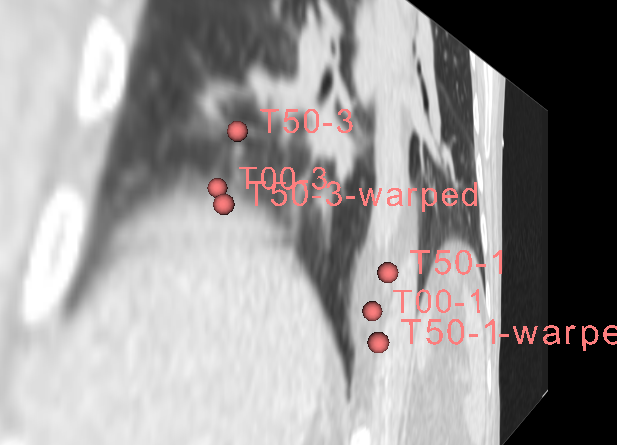
\includegraphics[width=0.9\textwidth]{./Images/landmark.png}
\caption{3D display of landmarks in three phases - T00 and T50 (end-inhale and end-exhale, respectively) and T50 warped to T00 (T50-warped). Average distance of corresponding landmarks between T00 and T50 is 0.1 and between T00 and T50-warped is 0.1.}
\label{inv}
\end{center}
\end{figure}


\subsubsection{Jacobian}
\label{Jacobian}

Jacobian determinant (Jacobian) of the vector field is used to validate physical behavior of registration \cite{Leow2007}. Jacobian of vector field should be positive, since negative Jacobian values correspond to folding, which is physically unrealistic for patient anatomy (organs can not be folded) \cite{Chen2008, Rey2002}. Expansions and contractions around a point are indicated by Jacobian values of greater and less than 1, respectively. 

DIRQA module calculates and displays the Jacobian of the vector field. Average, standard deviation, minimum and maximum values of Jacobian are also displayed. Similar to absolute difference it also has ROI feature implemented.

\begin{figure}[H]
	\begin{center}		
		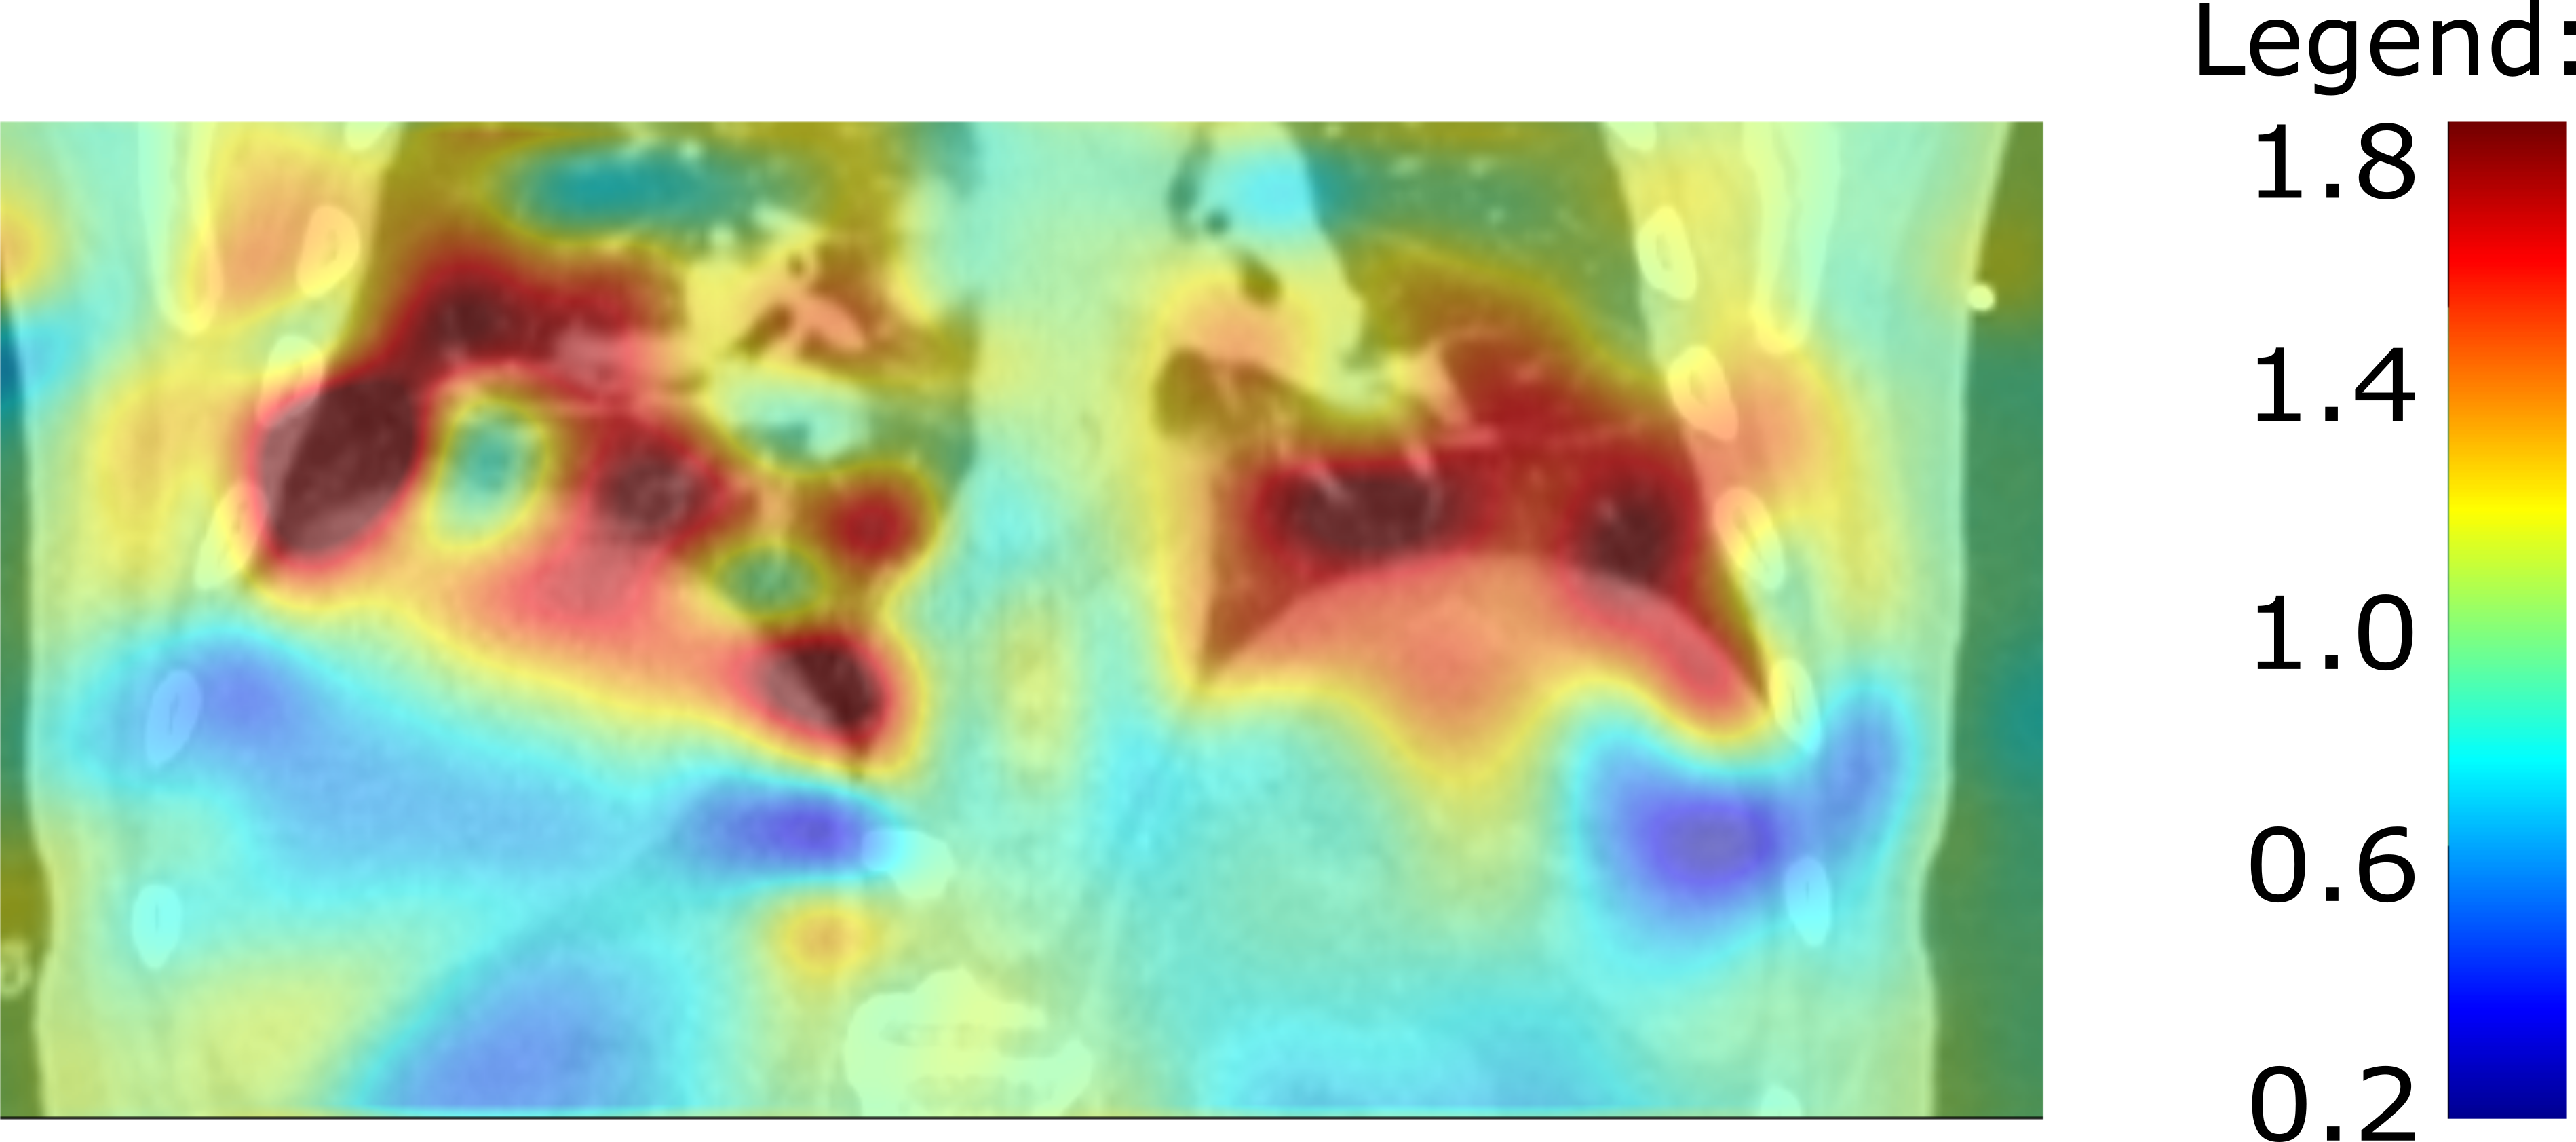
\includegraphics[width=0.9\textwidth]{./Images/jacobian.png}
		\caption{Image of Jacobian overlayed on CT scan. The average value of displayed Jacobian is 1.0 with 0.7 STD. \textbf{CHECK!}}
		\label{Jacobian}
	\end{center}
\end{figure}

\subsubsection{Inverse Consistency Error}
\label{ICE}

Inverse consistency error (ICE) is consistently used in literature as one of the main vector field checks \textbf{citati}. The principle is as followed. Suppose we have two vector fields - $u_{AB}$ obtained from registration of image A to B and $u_{BA}$ from registration of image B to A. The two registrations
should be preformed seperately. In ideal scenario, $u_{AB}$ would be a direct inverse of $u_{BA}$. However, deformable image registration algorithems do not yield perfectly inverse consistent vector field.

To check for ICE, an algorithm was created that first transforms point $x$ using $u_{AB}$. Newly obtained point $x'$ is then transformed with inverse vector
field, $u_{BA}$ which yields $x''$. The ICE is defined as Euclidean norm between $x$ and $x''$:

\begin{equation}
\label{eq:ice}
ICE = x - x'' = x - u_{BA}(x') = x - u_{BA}(u_{AB}(x))
\end{equation}

Points $x'$ and $x''$ can have an arbitrary position in space, while vector fields $u_{AB}$ and $u_{BA}$ are positioned on a grid. To apply transformation $u_{BA}(x')$ a interpolation has to be made to put $x'$ on a $u_{BA}$ grid. A tri-linear interpolation is used in this module.

As in Jacobian, ICE image is calculated and displayed, along with values for average, standard deviation, minimum and maximum values. ROI feature is also implemented. An example is shown in Fig.~\ref{inv}

\begin{figure}[H]
\begin{center}
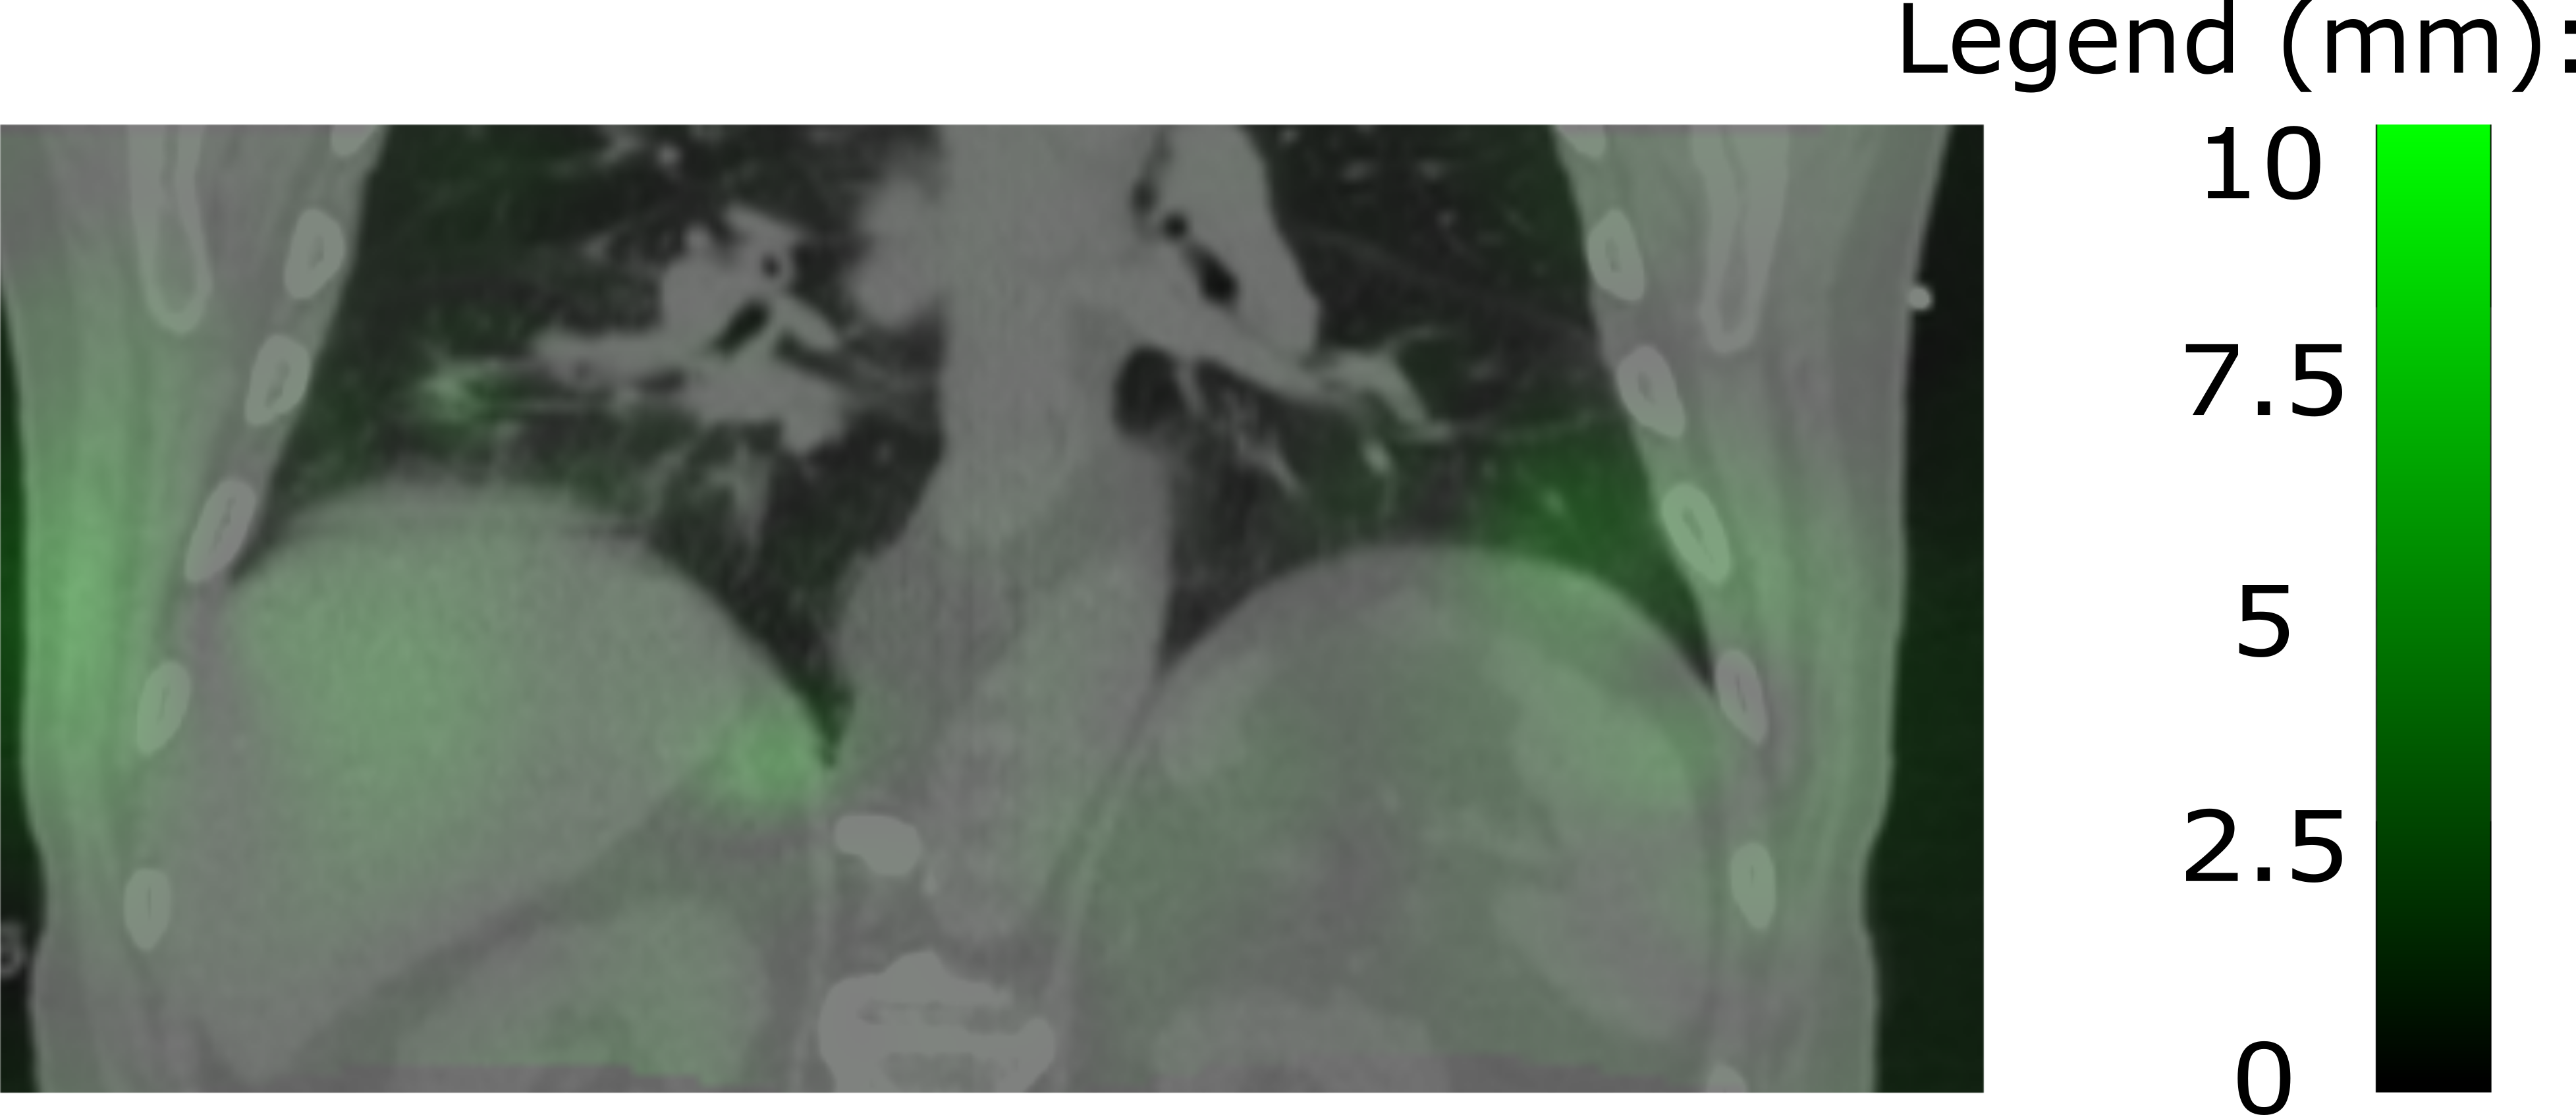
\includegraphics[width=0.9\textwidth]{./Images/inv.png}
\caption{Image of inverse consistency error (ICE) overlayed on CT scan. The average value of displayed ICE is 1.0 with 0.7 STD. \textbf{CHECK!}}
\label{inv}
\end{center}
\end{figure}


% \subsubsection{Output file}
% 
% With all different features to validate DIR it can be time consuming to go through them all. A special option was created to automatically go through all different validation steps. Furthermore it can also run through different phases, if there are more phases (i.e. in 4DCT). All produced data from DIR validation is stored on disk and can be reexamined by user upon request. Furthermore, images are created and data is summed up and displayed in a separate file. Users can then preview file for first validation of DIR and then open necessary files, if required.

% \subsection{Contour visualization}
% \label{Contour}
% 
% TRiP4D (see Section \textbf{REF}) introduced volume datasets for contour representation \cite{Richter2012}. It enabled necessary tasks for 4D calculations, such as the storing contour in different 4D states, contour propagation, etc. However, there was a lack of a proper visualization tool. In order to provide a contour visualization tool, a Slicer module was created. 
% 
% Contours are saved as volumetric boolean masks. A single bit per ROI contour representation marks each voxel inside volume dataset \cite{Richter2012}. To properly display contour, first a whole volume dataset was imported in Slicer. User selects which motion state he would like to inspect. The corresponding bit is then selected on the imported volume dataset. Lastly the contour is converted into 3D model shape. 
% 
% \subsection{Motion estimation and ITV creation}
% 
% ITV is often created by an eye investigation of all 4DCT phases, where the extent of motion is estimated. Automatic creation of ITV is scarce in commercial system, since it requires DIR on all 4DCT phases. A Slicer module was created to assist with the motion estimation and automatic ITV creation using DIR. 
% 
% Module is able to estimate and display motion of a user selected contour in three axis (left-right, anterior-posterior, superior-inferior) based on DIR vector fields. Module also performs DIR on 4DCT with patient hierarchy, if it has not been done yet.
% 
% Beside motion estimation, module can also propagate selected contour (usually CTV) and propagate it to all 4DCT and make a convolution of all propagated contours, resulting in automatically generated ITV.
% 
% \subsubsection{Generation of mid-position phase}
% 
% Most commercial software calculates treatment plan on a single 3D CT scan, using 4DCT only for motion estimation. To incorporate patient-specific motion information, a 3D CT scan was created from 4DCT in the time averaged position, also known as mid-position scan (midP scan) \cite{Wolthaus2008}. With midP scan commercial software can still be used. Additionally, it also enabled smaller error margins for PTV generation and midP scan has less noise as individual 4DCT scans, because it uses more data. 
% 
% Construction of a midP begins with registration of whole 4DCT. The resulting vector fields from reference position to 4DCT phases are then averaged to obtain mean vector field, see Fig.~\ref{midPgeneration}. Afterwards, for each vector field the mean vector field was subtracted, yielding a set of mean-corrected vector fields pointing from mean position to corresponding 4DCT phase. The mean-corrected vector fields were finally inverted and applied to each 4DCT phase, resulting in each phase being in the same, time-averaged position. In the end the set of transformed 4DCT phase was averaged to obtain midP scan.
% 
% \begin{figure}[H]
% \begin{center}
% 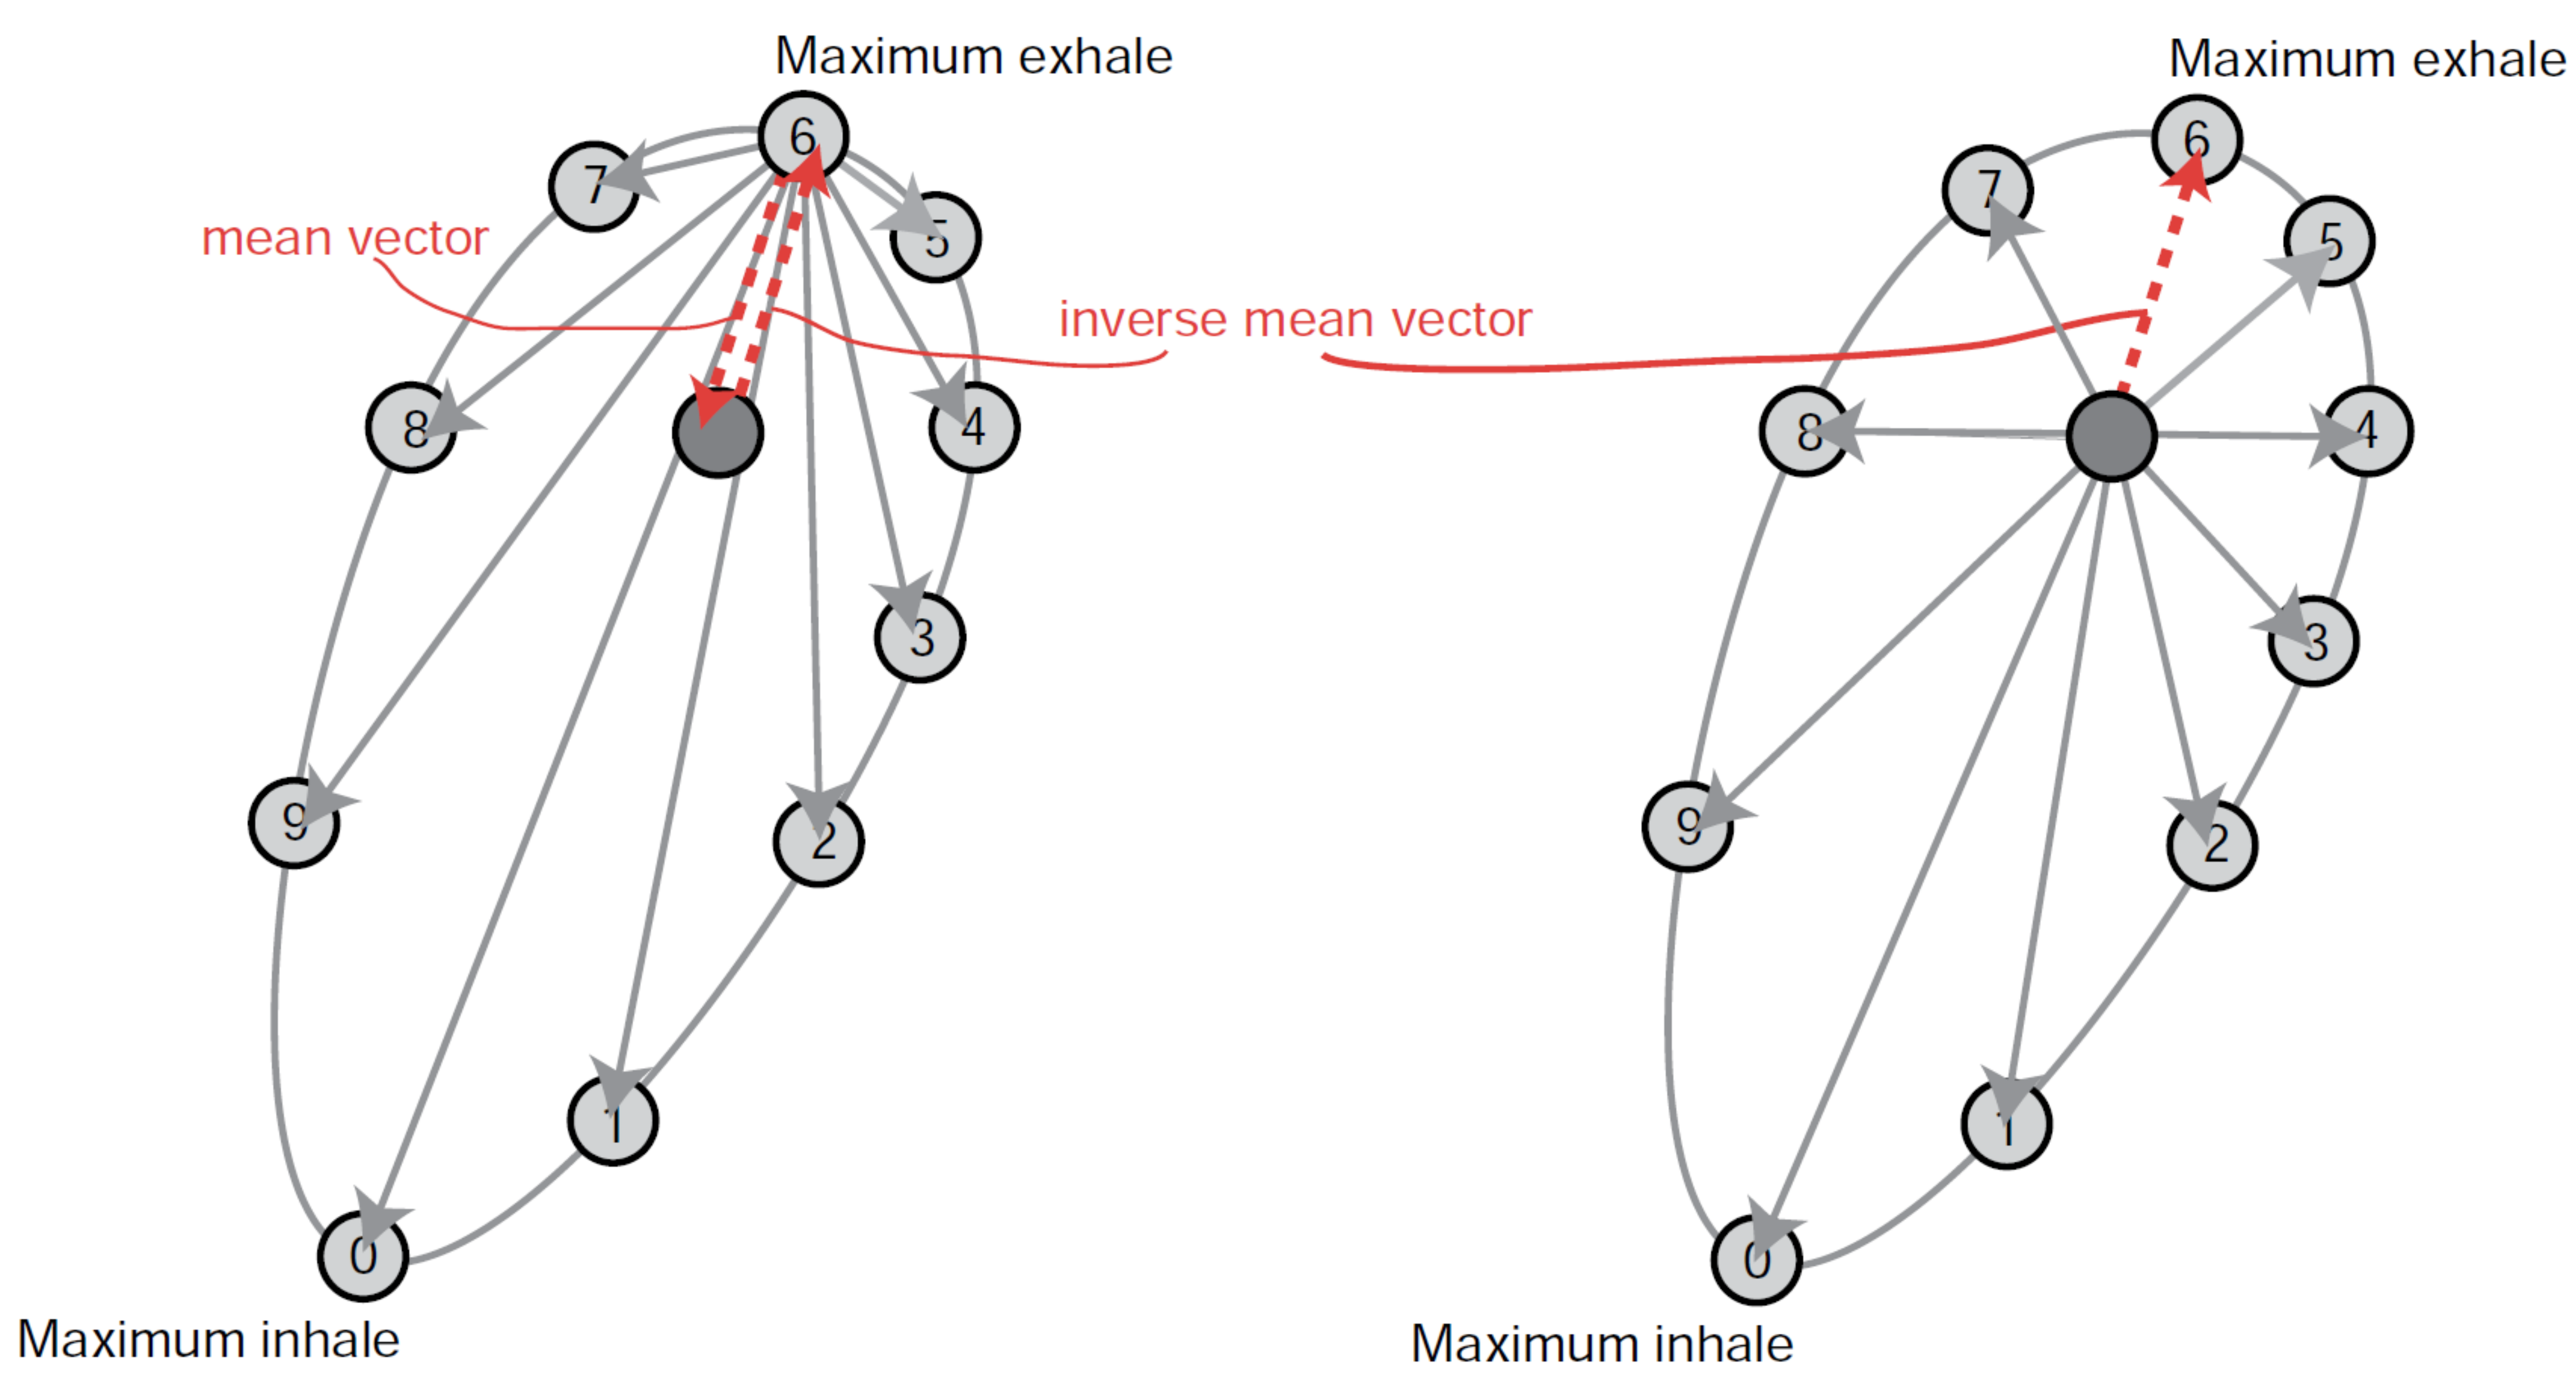
\includegraphics[width=0.9\textwidth]{./Images/midPgeneration.png}
% \caption{Computation of the midP scan. All vectors have the same starting point (reference phase, maximume exhale in the this example), therefore they can be averaged, resulting in the mean vector.
% 	Next vectors from mean position to 4DCT phases have to be computed, which is achieved by substracting original vectors and mean vector. Figure taken from \cite{Wolthaus2008}}
% \label{midPgeneration}
% \end{center}
% \end{figure}


\newpage
\section{Verification}
\label{Verification}

Several extensions for Slicer were created to tackle the issue of motion in treatment planning. With these extensions it is possible to preform DIR, DIR quality assurance, estimate organ motion and make midP scans. All extensions have to be checked on actual clinical data, to make future extension usage possible. Furthermore it is necessary to test if extensions could be used in a typical clinical workflow. Especially DIR validation, which is the reason for the lack of DIR in commercial treatment planning software. 

DIR and DIR validation was done on lung 4DCT patient data. As part of a GSI pig-irradiation project (?) DIR and DIR validation was integrated in clinical workflow. Finally an example of midP scan on a liver cancer patient and it's usage will be presented.

\subsection{Registration of lung 4DCT patient data}
\label{lungDIR}

Chapter \textbf{REF} and \textbf{REF} present studies on simulating active scanning carbon ion treatment (CiT) for lung cancer patient. The effects of interplay can drastically chage the dose distribution for CiT and it is necessary to quantify effects of motion with DIR and transfer results into
treatment planning software (TRiP4D in this case). An automatic procedure is required to preform DIR and DIR validation on a large number of patients. This was achieved with Slicer modules described in Section~\ref{Implementation}.

\subsubsection{Materials and Methods}

A a time-resolved CT (4DCT), consisting of 10 motion phases (0\% - 90\%) with resolution \textbf{?} was aquired for 23 patients.
Phase 0\% corresponds to an end-inhale phase and was chosen as a reference phase.

DIR was preformed for each patient between each phase and reference phase and vice verse (true DIR and inverse DIR). For each patient 18 registrations were made, leading to 414 registrations in total.

DIRs were done with B-Spline Plastimatch module and patient hierarchy in Slicer (see Section~\ref{Registration} and \ref{PatHierarchy}). Two stages were used with details given in Table~\ref{tab:stages}. 

\begin{table}[H]
  \centering
%   \footnotesize
  \caption{Parameters used for Plastimatch registration. A mean squared error metric was used. Details for each parameter can be found in \cite{Plastimatch}.}
  \begin{tabular}{c|c|c}
      Parameter & Stage 1 & Stage 2 \\
      \hline
      Resolution & 4,4,2 & 1,1,1 \\
      Grid size & 50 & 15 \\
      Regularization lamda & 0.005 & 0.005 \\
      Iterations & 200 & 100 \\
    \hline\hline
  \end{tabular}
  \label{tab:stages}
\end{table}

Absolute difference was computed for three image pairs: reference and moving image (default absolute difference), reference and moving warped image (true absolute difference), moving and reference warped image (inverse absolute difference). In total 621 absolute differences were caluclated and a down-sampling by a factor of 2 was
done on all images before calculation to save computer time. Similarly, 414 vector fields were also down-sampled by a factor of 2 before calculating Jacobian and ICE checks.

ROI around patient body was manually created to get better results - area outside of patient is roughly the same in all states (air) and does not contribute to DIR. ROI was then used in absolute difference, Jacobian and ICE.

For each patient it took around 1 h for all 20 DIR and \textbf{30 min} for complete DIRQA on all 20 DIR  on Linux computer with 8 clusters and 16 GB RAM.


\subsubsection{Results}

DIR was successfully performed on all 23 patients. An example of DIR is shown on Fig.~\ref{exampleReg_lung}. Vector fields resulting from all DIR were analyzed and data is shown in Table~\ref{tab:vectordata_lung}. There was no statistical
difference between true and inverse vector fields. The biggest contribution to vector field magnitude was from superior-inferior direction (around 50\%), next was anterior-posterior direction (around 30\%) and the smallest contribution was from left-right direction (around 20\%).

\begin{table}[H]
  \centering
%   \footnotesize
  \caption{Data of vector magintudes. Values are presented as average (range).}
  \begin{tabular}{c|c|c}
  
       & True vector field & Inverse vector field  \\
       \hline
       Mean & 0.38 (0.01 - 1.28) & 0.38 (0.01 - 1.3) \\ 
       STD & 0.95 (0.04 - 3.17) & 0.98 (0.04 - 3.55) \\ 
       Max & 9.67 (0.61 - 28.56) & 10.17 (0.56 - 37.11) \\
    \hline\hline
  \end{tabular}
  \label{tab:vectordata_lung}
\end{table}

Dependence of true and inverse absolute difference on default absolute difference is shown in Fig.~\ref{absDiff_lung}. Fig.~\ref{absDiff_lung} also shows default absolute difference distribution accross 9 phases. 

Distribuition of Jacobian and ICE results are shown in Fig. \ref{jacobian_data} and \ref{ice}. Maximum values of true and inverse maximum and minimum Jacobian and ICE were tested against maximum vector magnitudes and fitted with linear function. Results are plotted in Fig.~\ref{maxvf}.
Additionally, dependence of maximum true Jacobian on minimum inverse Jacobian was tested and results are display in Fig.~\ref{calcJac_lung}. Parameters from linear fit in Fig.~\ref{calcJac_lung} were used to calculate so-called scaled Jacobian for outliers. Each voxel, $x$, in scaled Jacobian, $S$ was calculated from true and inverse Jacobian, $J_{True}$ and $J_{Jacobian}$, as:

\begin{equation}
S(x) = 1.7 ln(J_{True}(x)) + ln(J_{Inverse}(x))
	content...
\end{equation}

Example of scaled Jacobian is shown in Fig.~\ref{calcJac_lung}.

All linear fits used in Fig.~\ref{absDiff_lung}, ~\ref{calcJac_lung} and ~\ref{maxvf} were statistically significant (p < 0.05).

\begin{figure}[H]
	\begin{center}		
		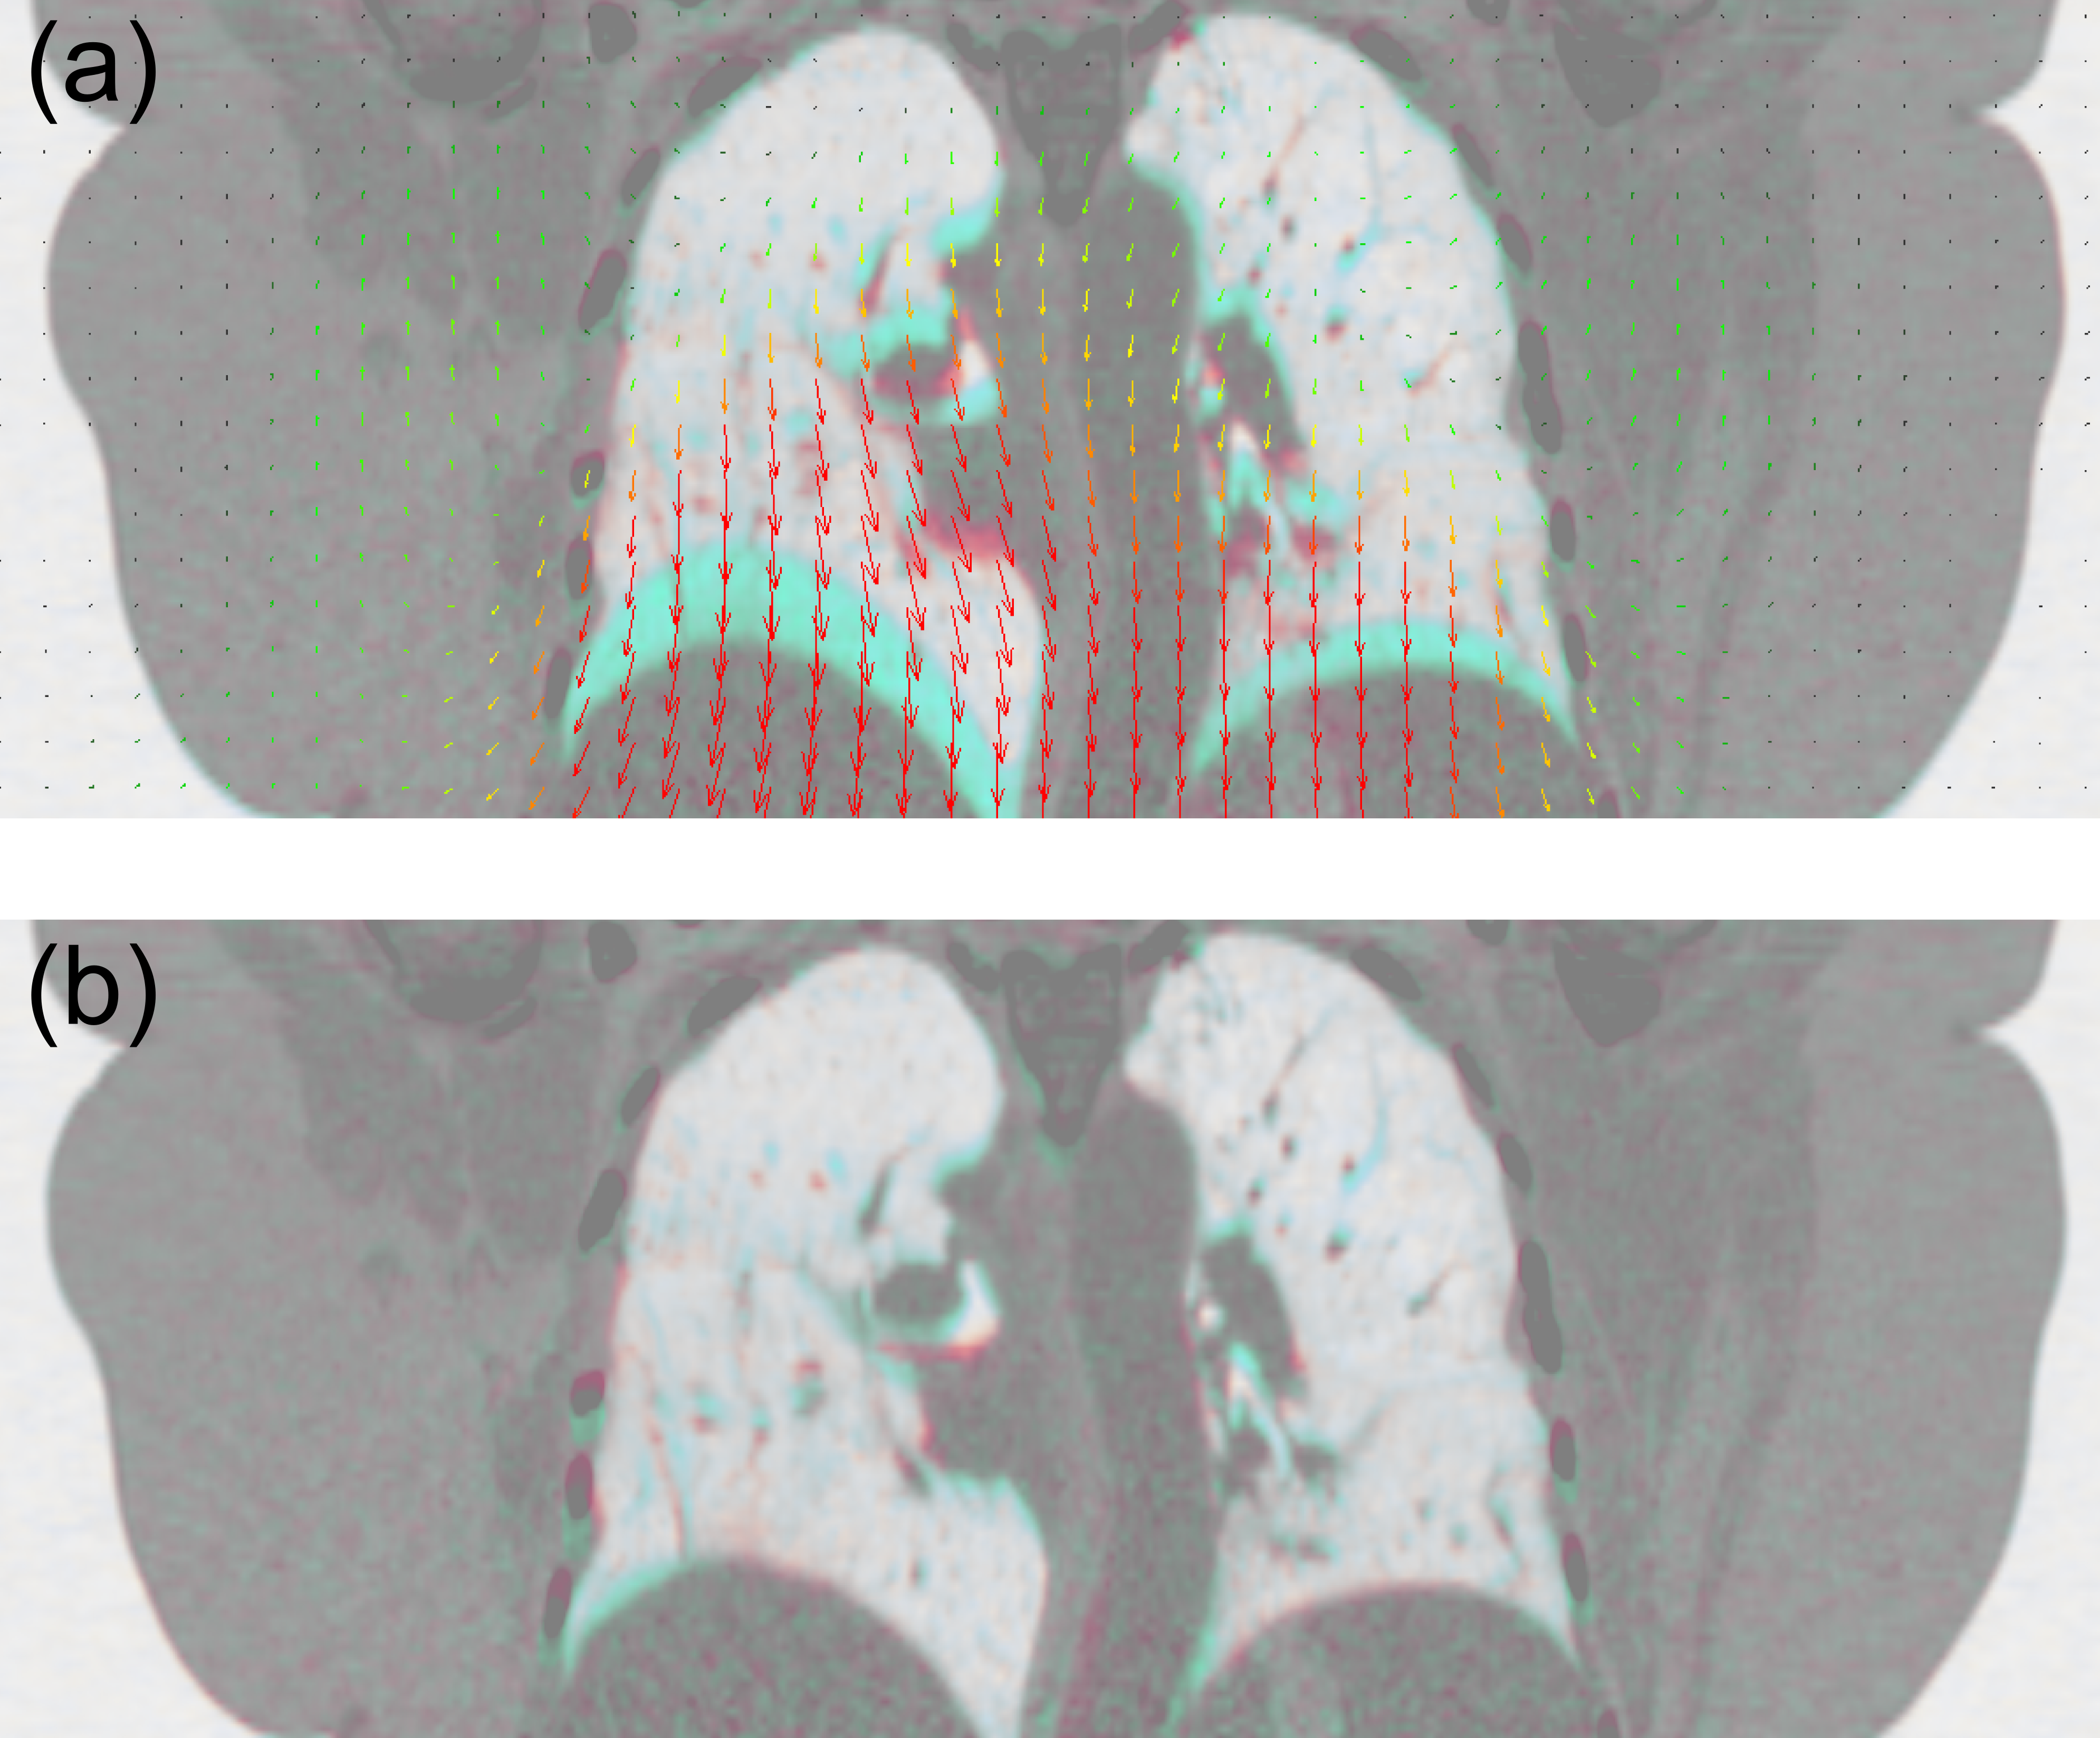
\includegraphics[width=0.6\textwidth]{./Images/exampleReg.png}
		\caption{False color overlay of two phases before (a) and after (b) DIR. Vector field is displayed on image (a) as arrows.}
		\label{exampleReg_lung}
	\end{center}
\end{figure}



\begin{figure}[H]
	\begin{center}		
		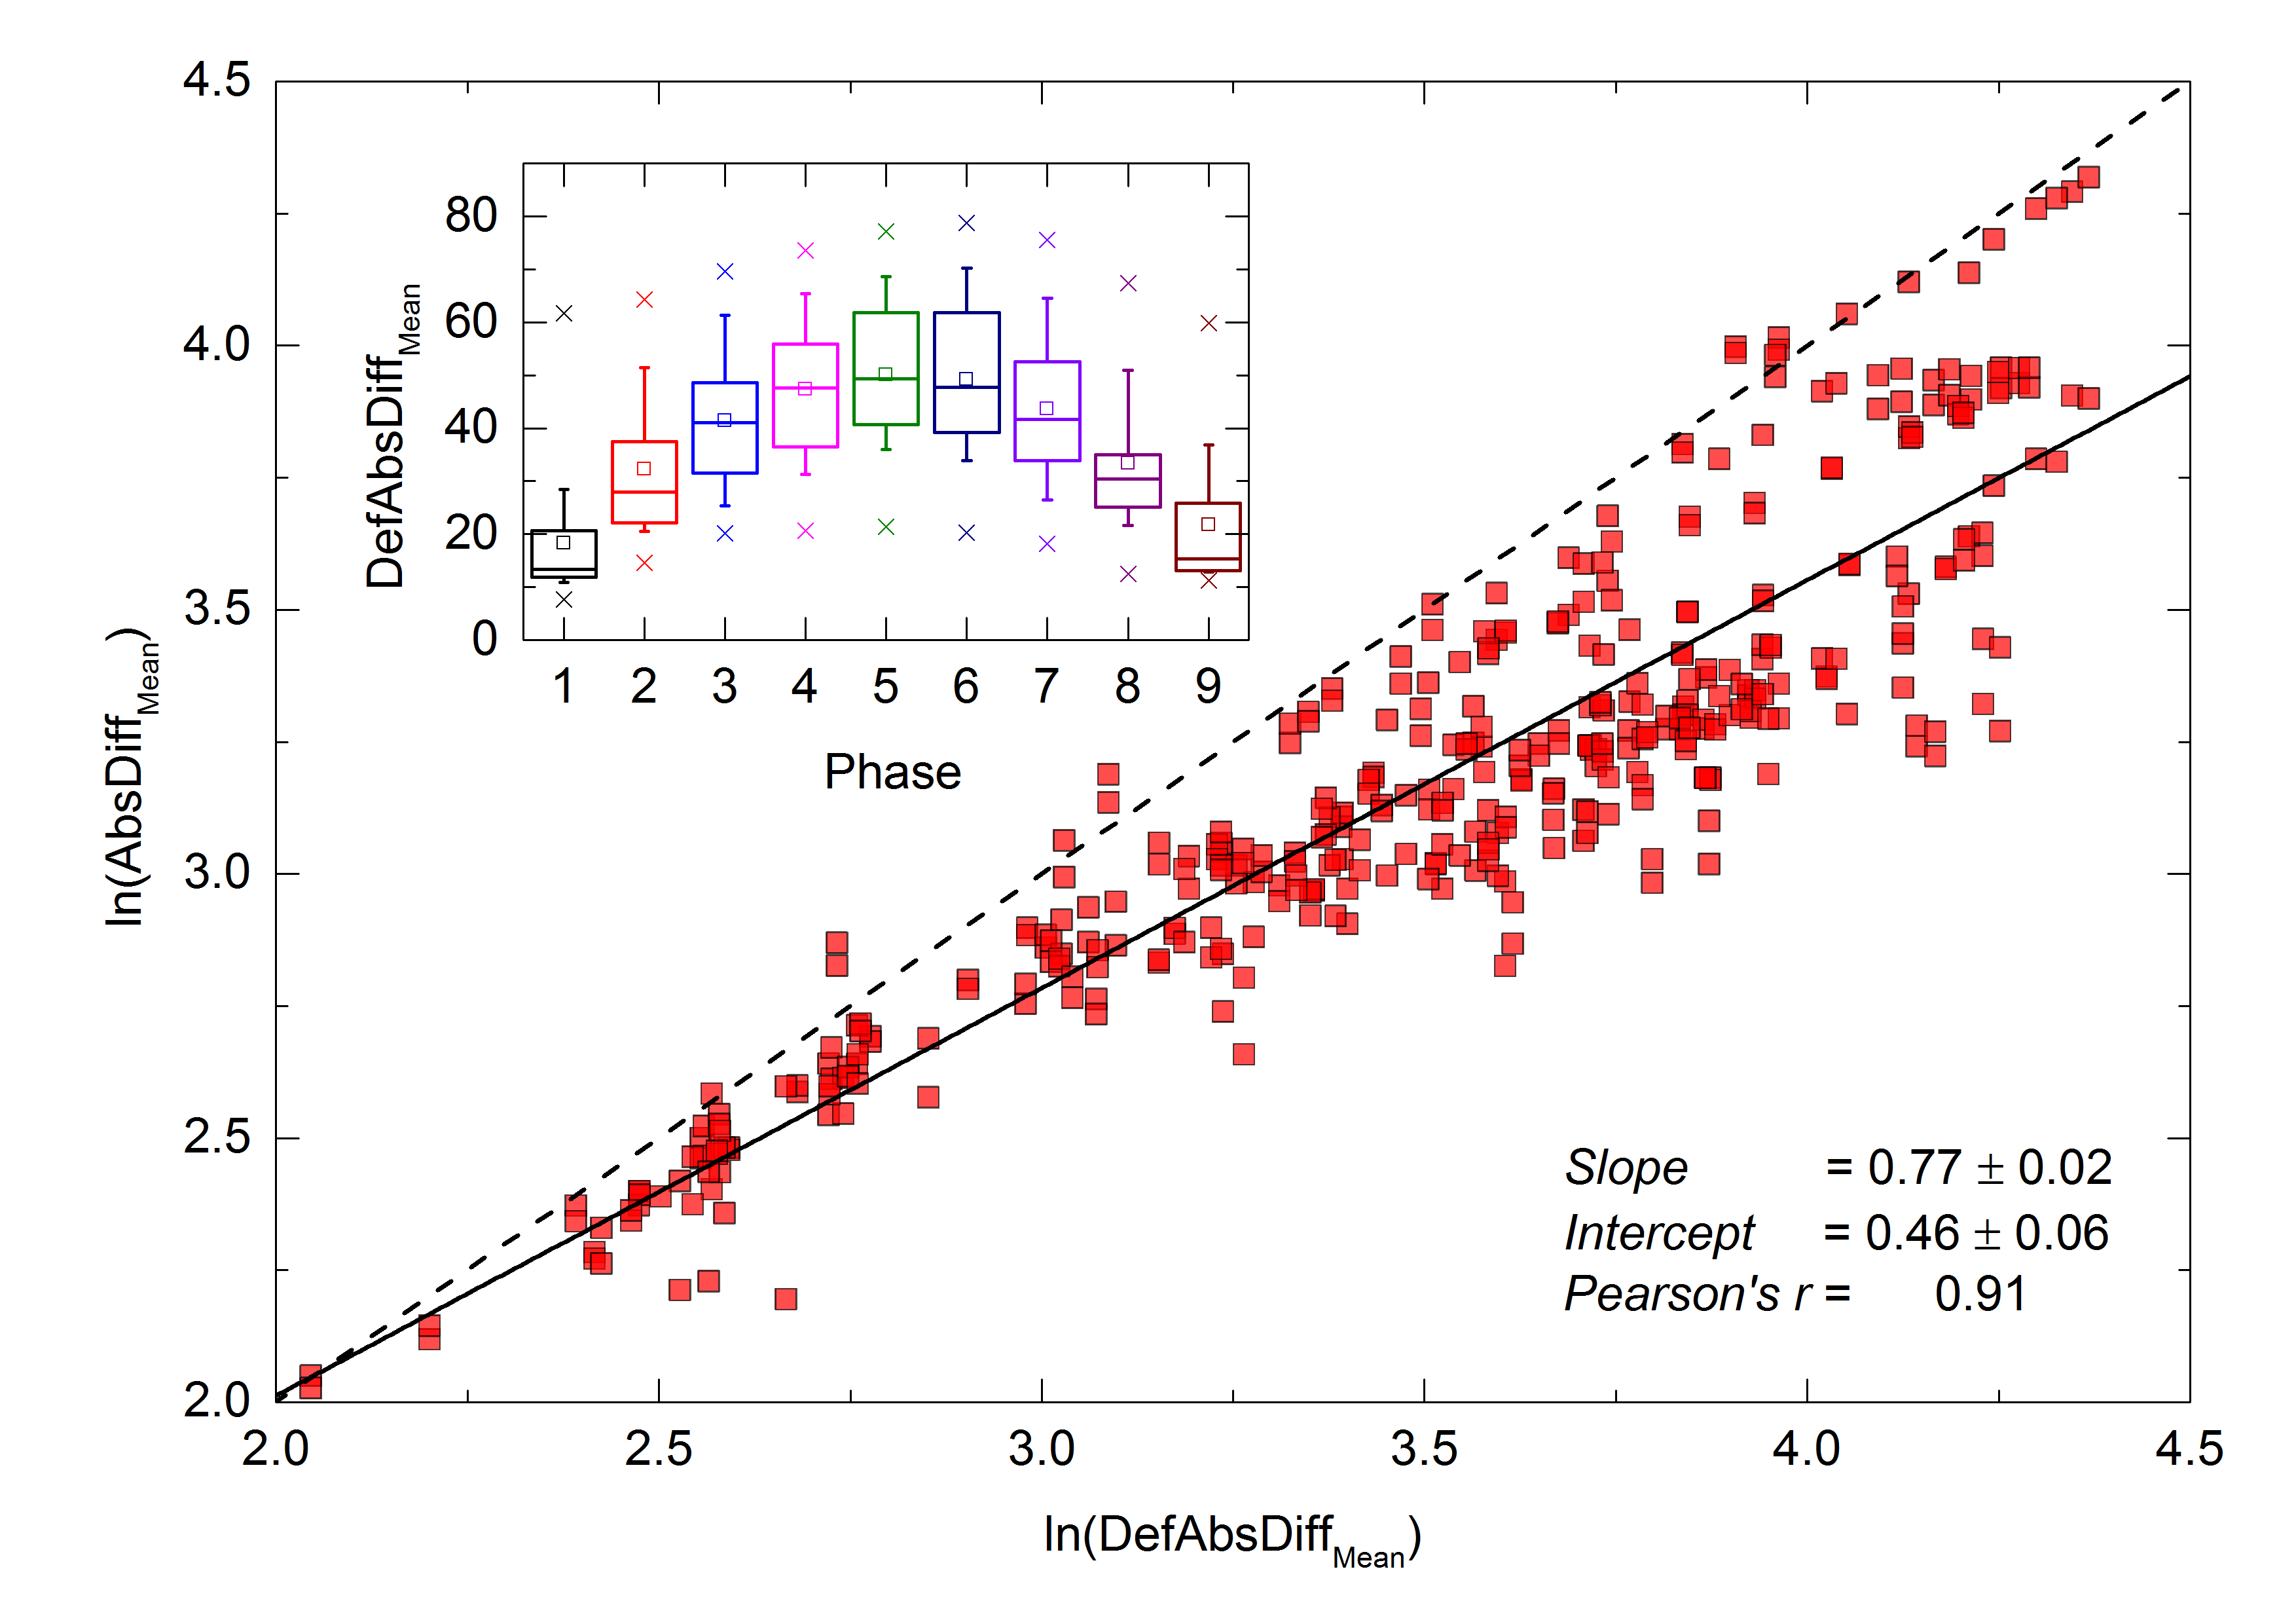
\includegraphics[width=0.7\textwidth]{./Images/absDiff.png}
		\caption{Natural logarithm of true and inverse absolute difference (AbsDiff) plotted against default absolute difference (DefAbsDiff). Solid line shows linear fit, with parameters
		writen in corner. Dashed line shows $y(x)=x$ plot. Inset shows box plots of mean distribution of default absolute difference across nine 4DCT phases. Boxes represent 25-75\%, whiskers 10-90\%
		of data, median is shown with solid line, mean with square and outliers with crosses.}
		\label{absDiff_lung}
	\end{center}
\end{figure}


\newpage

\begin{figure}[H]
	\begin{center}		
		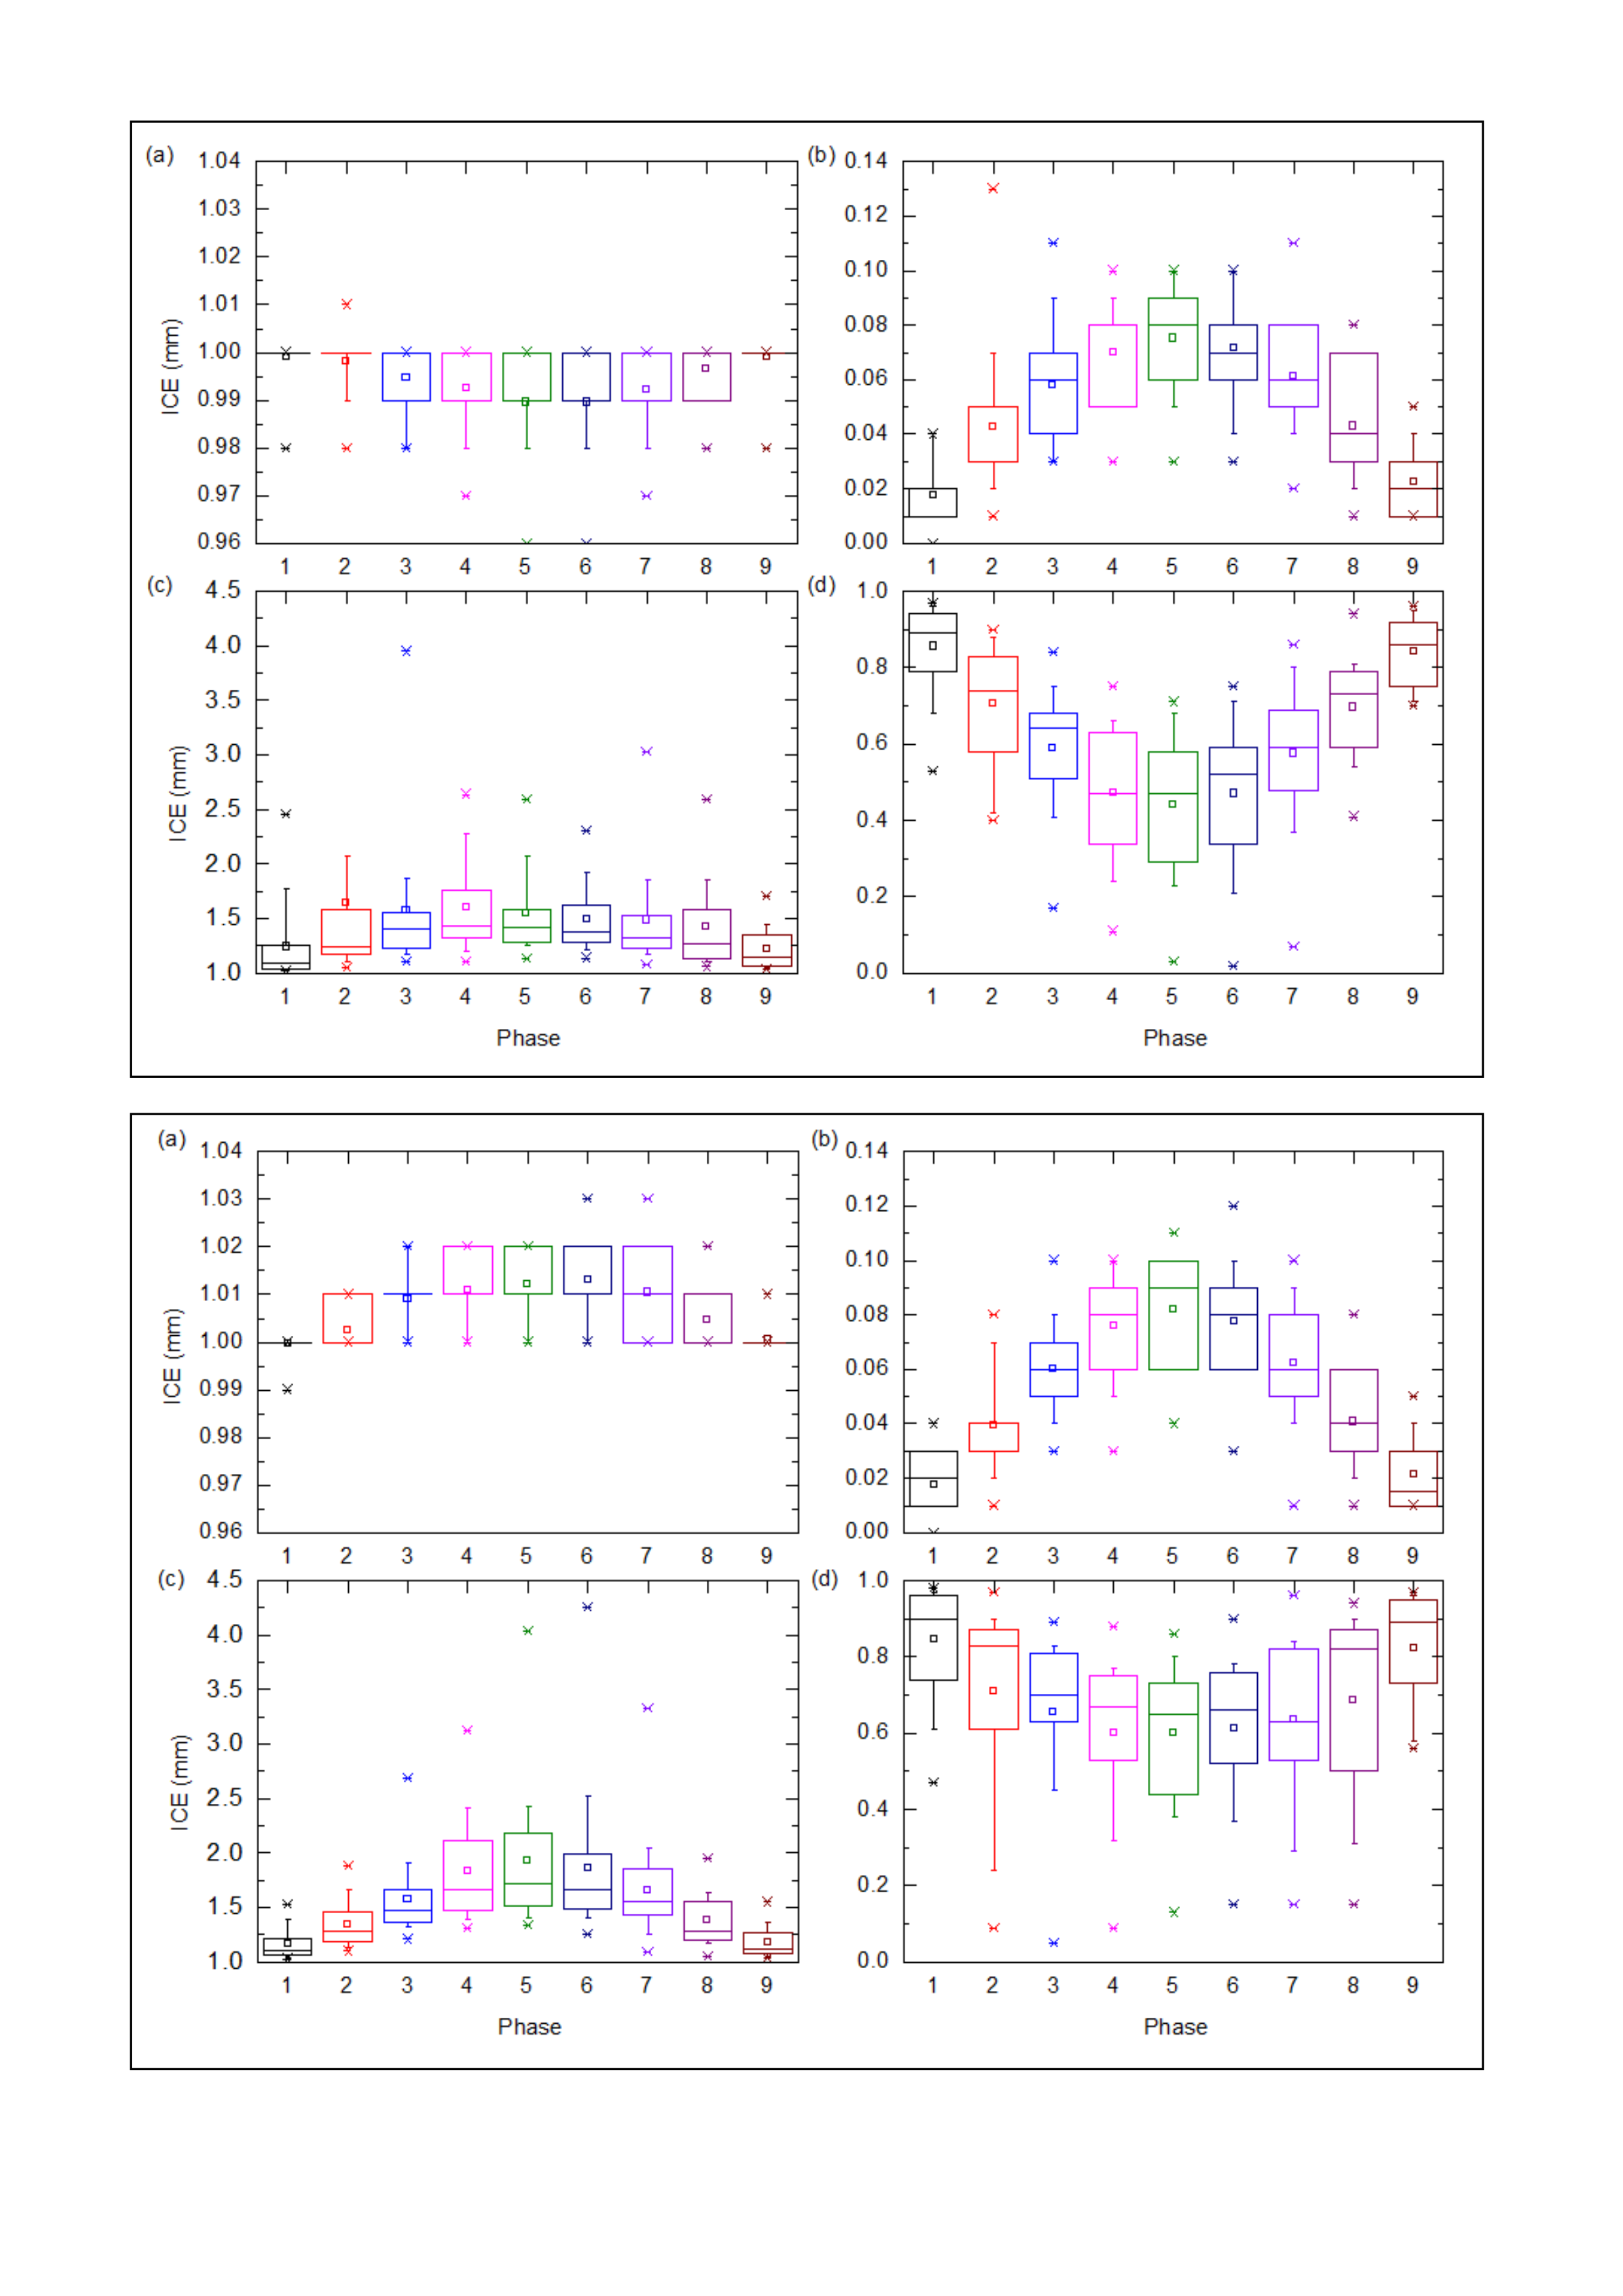
\includegraphics[width=0.75\textwidth]{./Images/Jacobian_data.png}
		\caption{Data for Jacobian of vector fields (top) and inverse vector fields (bottom) for 9 4DCT phases (reference phase 0 is excluded) for 23 lung cancer patients. Mean, STD, maximum and minimum are represented as (a), (b), (c) and (d), respectively.
		Boxes represent 25-75\%, whiskers 10-90\% of data, median is shown with solid line, mean with square and outliers with crosses.}
		\label{jacobian_data}
	\end{center}
\end{figure}

\newpage

\begin{figure}[H]
	\begin{center}		
		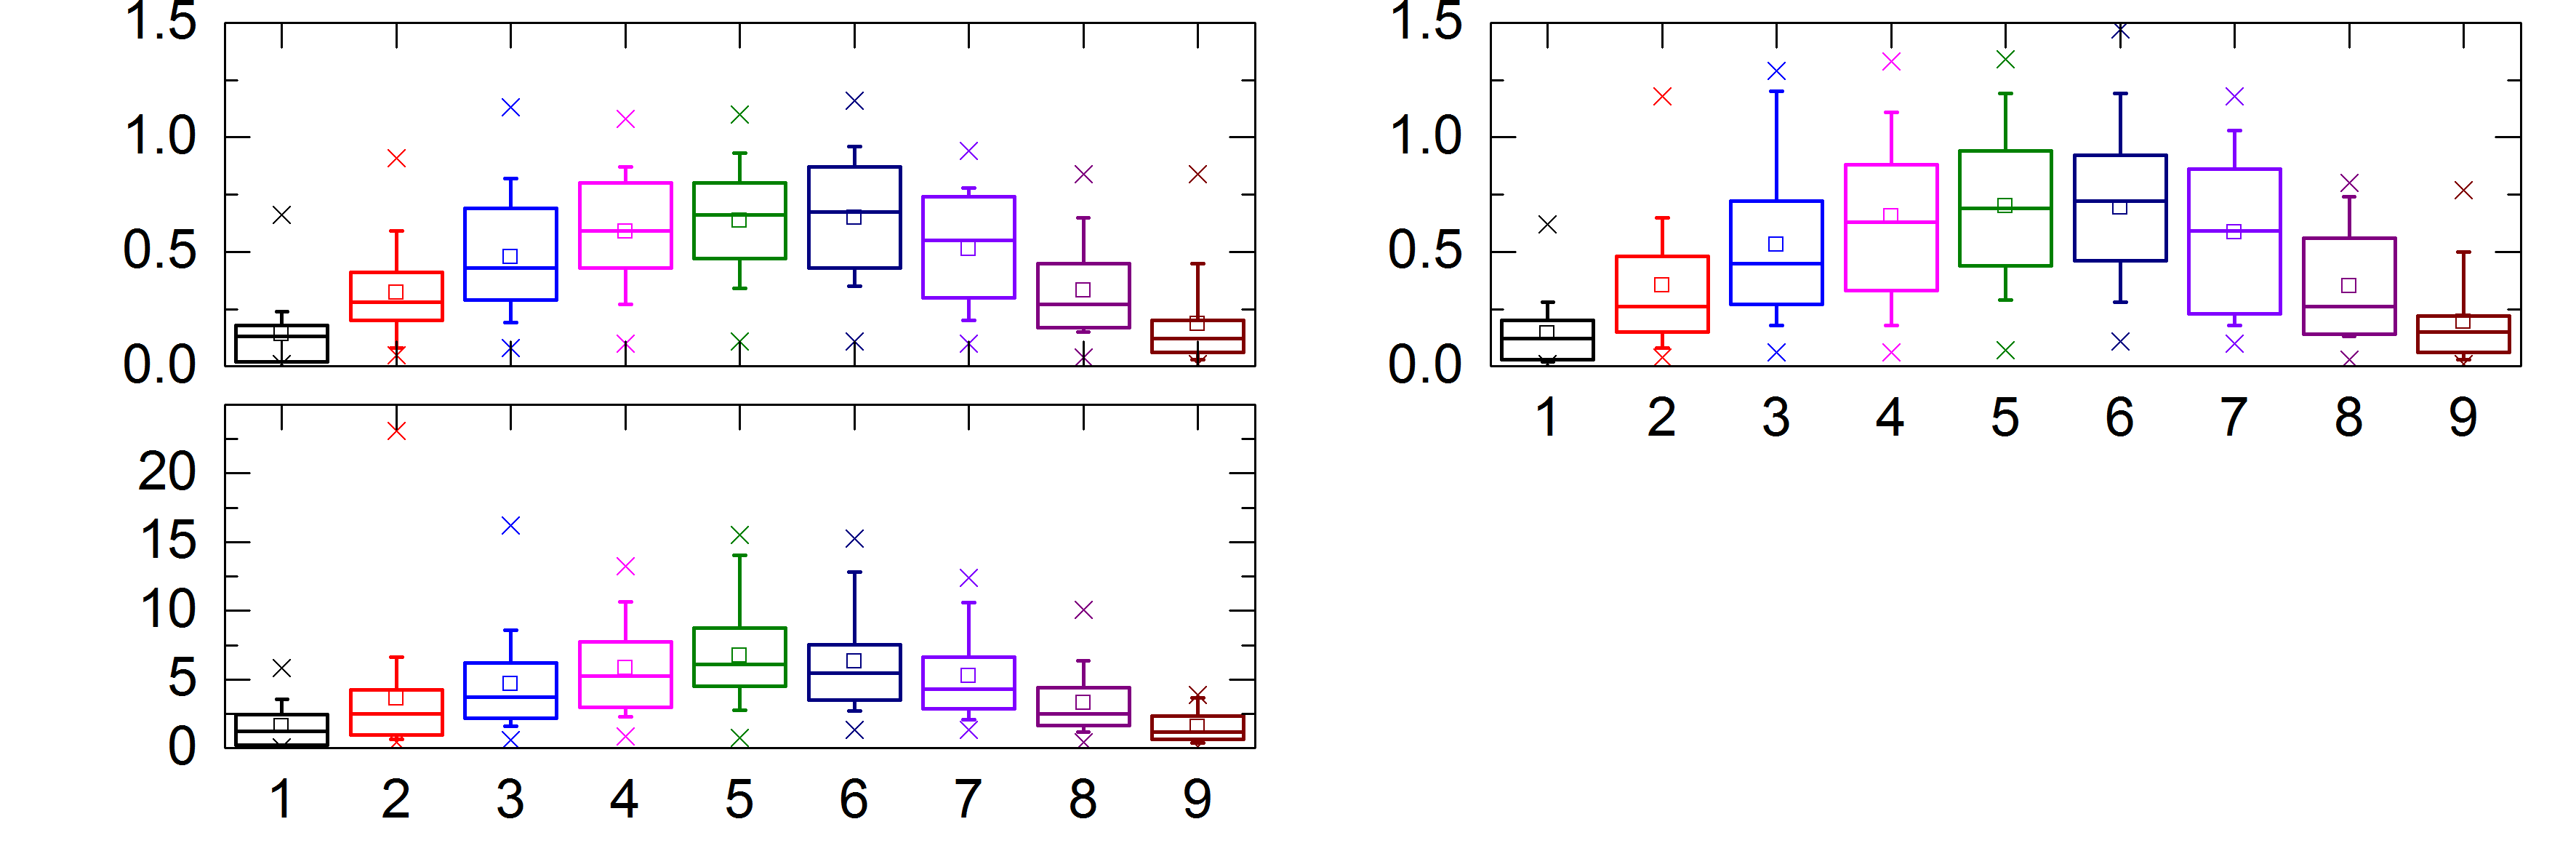
\includegraphics[width=0.9\textwidth]{./Images/ICE.png}
		\caption{Data for ICE for 9 4DCT phases (reference phase 0 is excluded) for 23 lung cancer patients. Mean, STD, maximum are represented as (a), (b) and (c), respectively. ICE Minimum is 0 throughout all phases and patients.
		Boxes represent 25-75\%, whiskers 10-90\% of data, median is shown with solid line, mean with square and outliers with crosses.}
		\label{ice}
	\end{center}
\end{figure}



\begin{figure}[H]
	\begin{center}		
		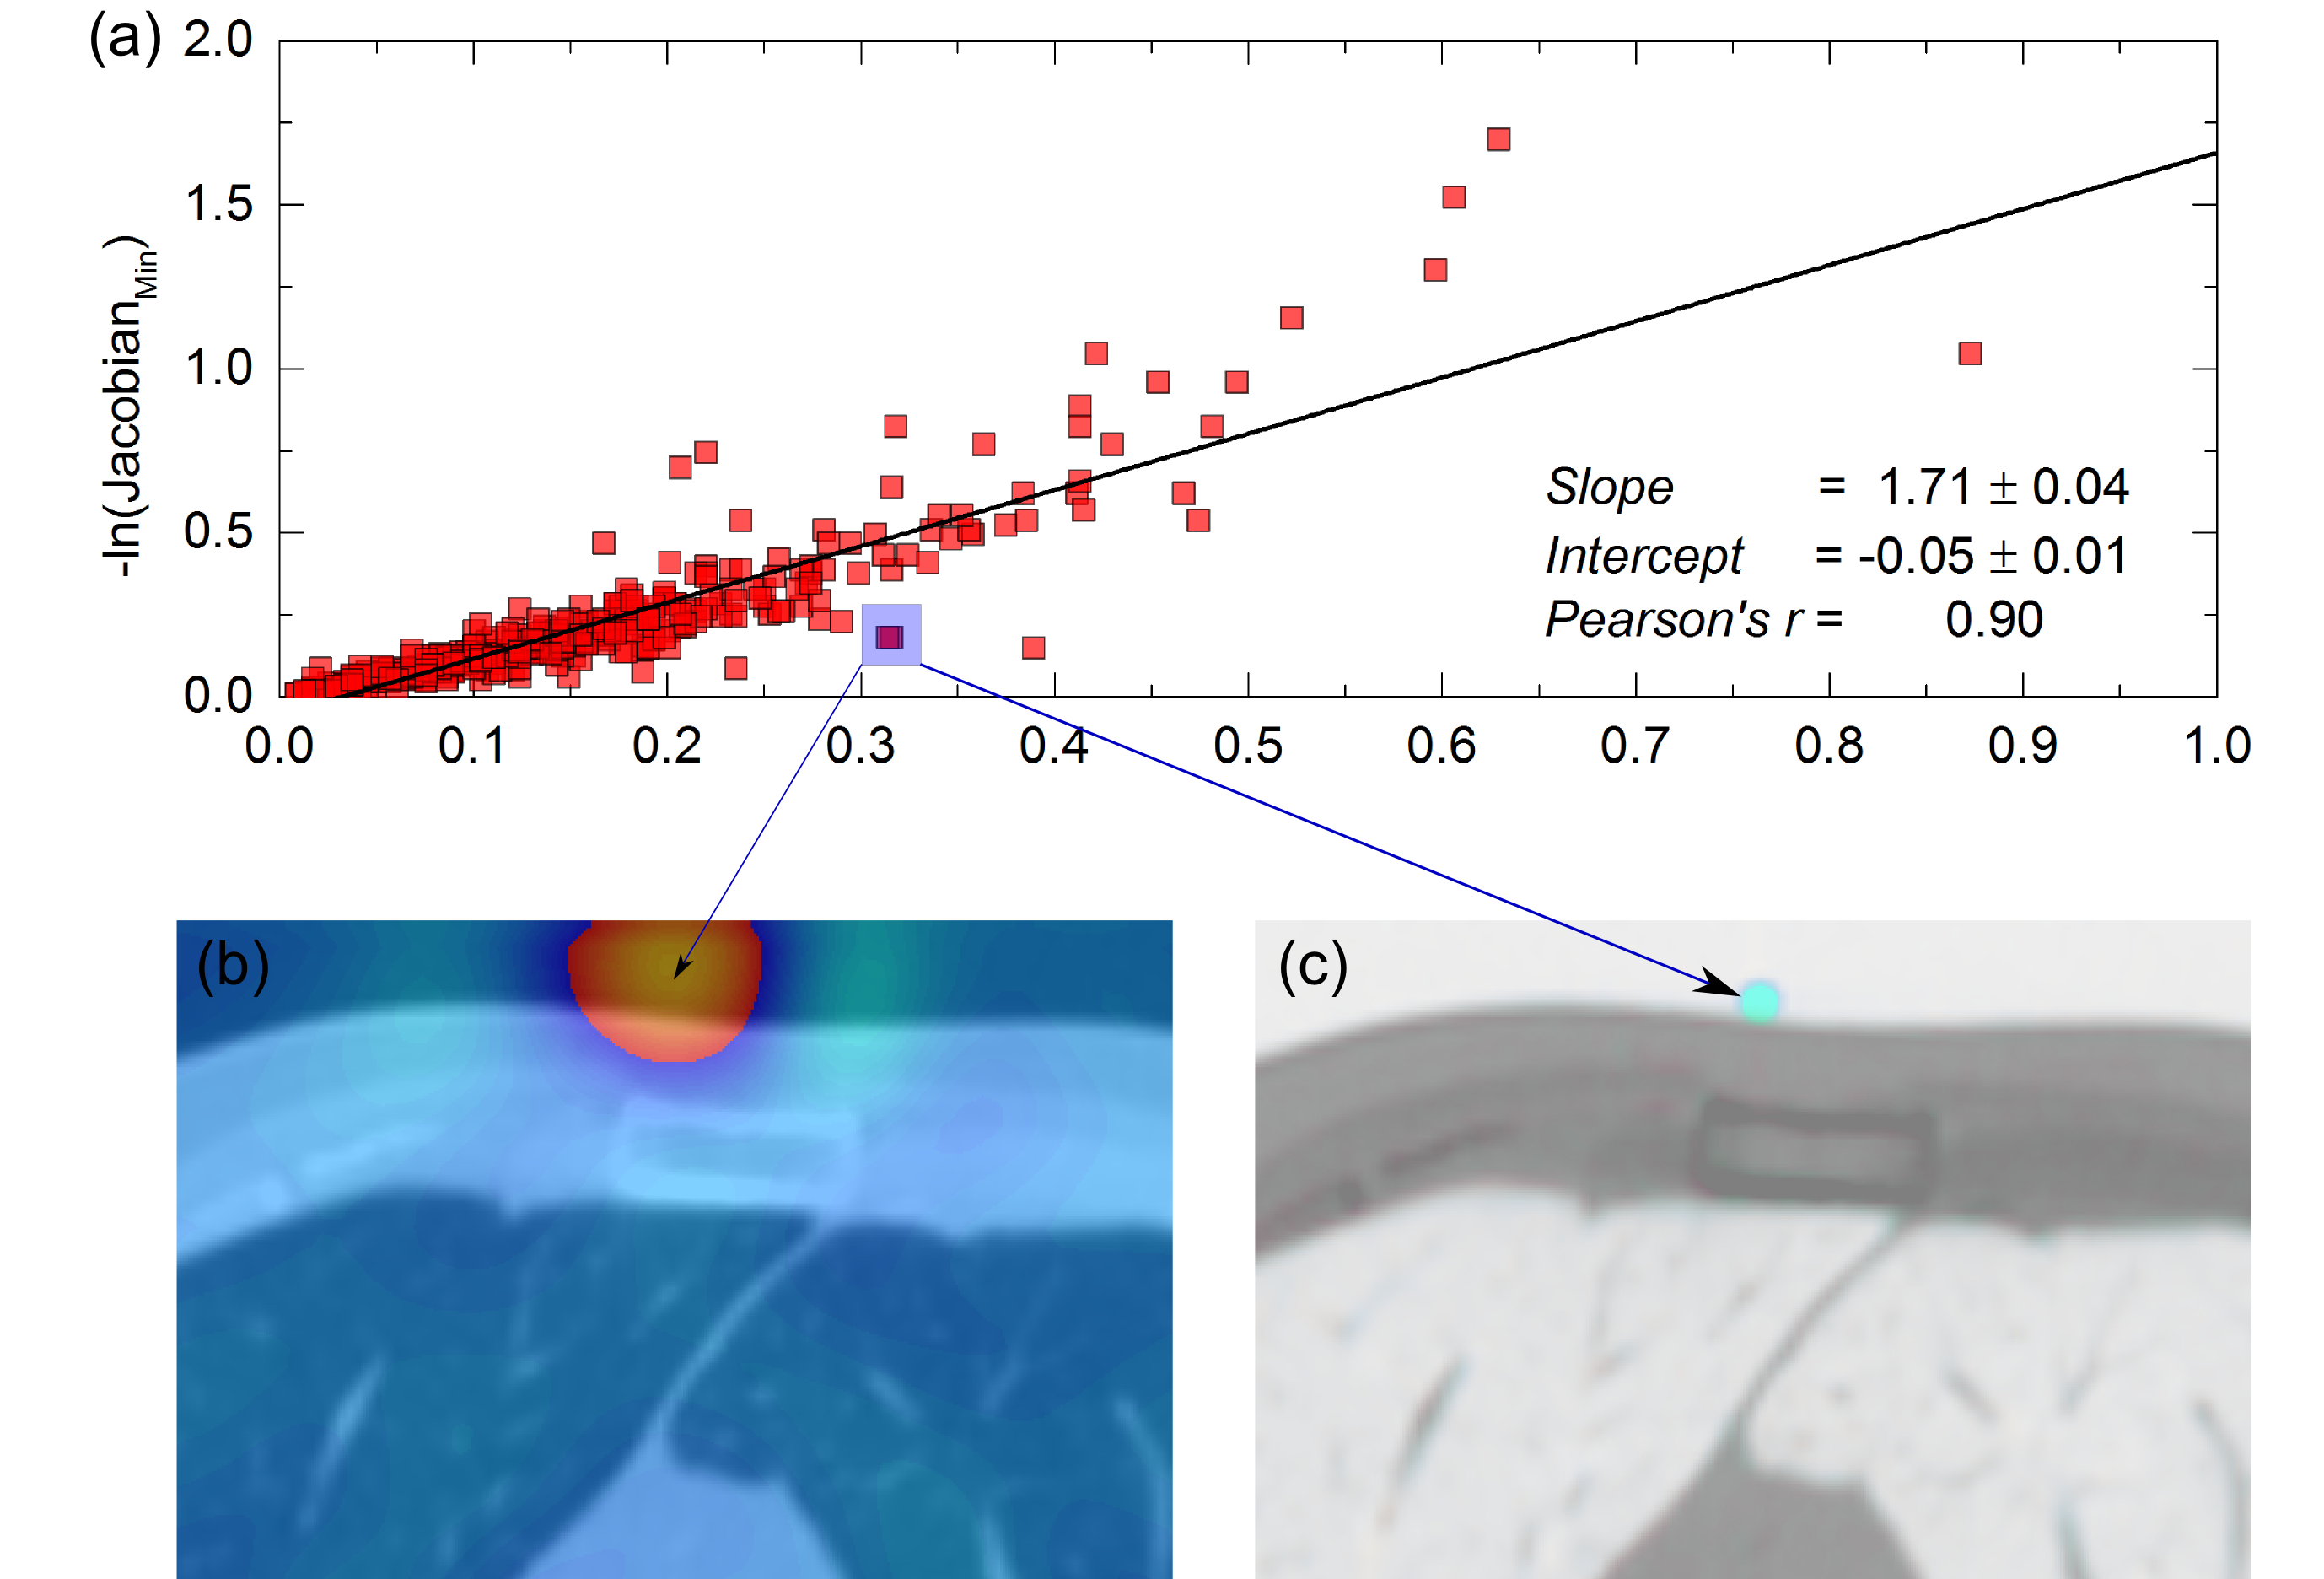
\includegraphics[width=0.8\textwidth]{./Images/jacSum_lung.png}
		\caption{(a) Plot of negative natural logarithm of minimum Jacobian versus maximum Jacobian. Linear fit is displayed with solid line and it's parameters are given in the corner. (b) Shows part of the image of modifed Jacobian (see text) overlayed on patient CT scan. (c) shows the CT scan of phases where Jacobian patient in (b) was calculated in false color.}
		\label{calcJac_lung}
	\end{center}
\end{figure}

\newpage

\begin{figure}[H]
	\begin{center}		
		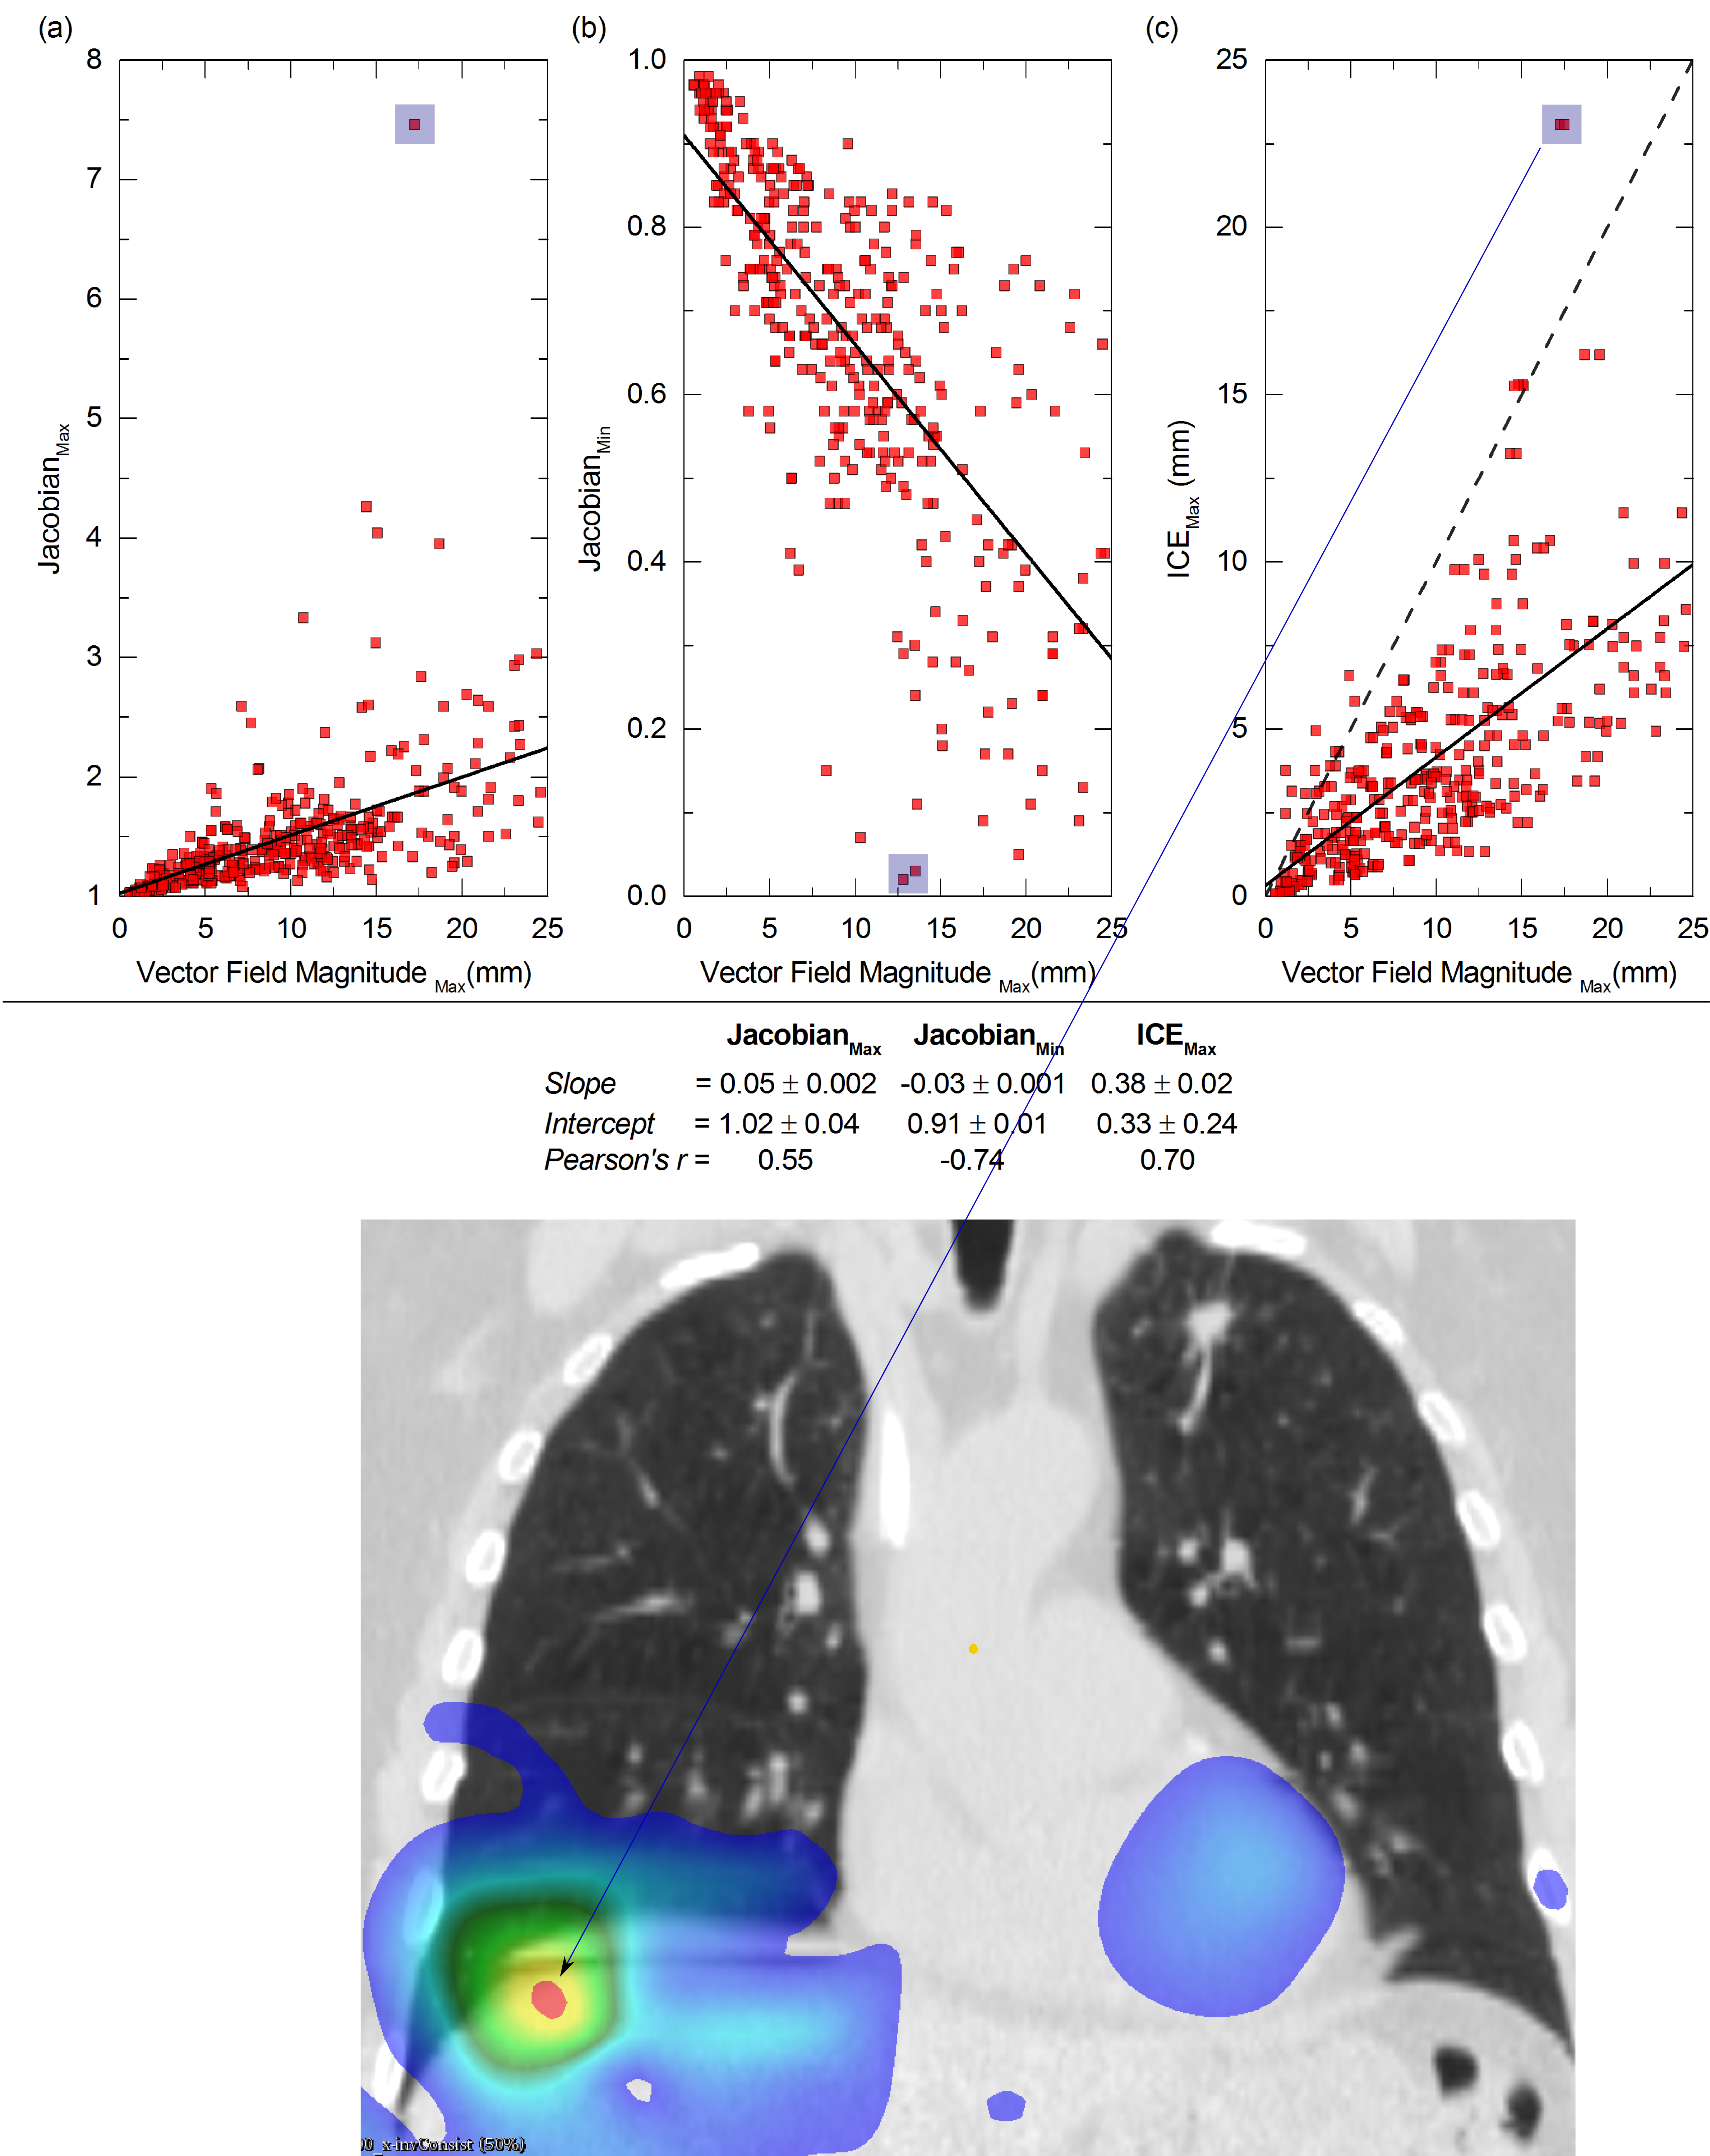
\includegraphics[width=0.9\textwidth]{./Images/maxVf_lung.png}
		\caption{Values of maximum Jacobian (a), minimum jacobian (b) and ICE (c) plotted against maximum vector magnitudes. Linear fit is displayed with solid line and parameters are written below the plots. Dashed line in (c) shows $y(x)= x$ plot. Values resulting from patient on image (d) are highlighted with blue squares in (a)-(c).
			ICE is displayed on (d) using color table as displayed in legend.}
		\label{maxvf}
	\end{center}
\end{figure}

\newpage

\subsubsection{Discussion}

Vector field magintudes confirms previously published data that the biggest motion for lungs is in superior-inferior direction \cite{Seppenwoolde2002, Britton2007, Liu2007}. The mean vector field magnitude is small (in submilimiter range), 
because the ROI included the whole patient body, not just the lungs where most of the motion occurs. Vectors and inverse vectors are similar, which was expected.

There was a good correlation (Pearsons's r = 0.91) between absolute difference before and after DIR. The greater the difference between reference and moving image, the better DIR can match them. Few cases
have sligthly higher absolute difference after DIR, which should not occour, since DIR was minimizing absolute difference metric. The reason lies in construction of warped images. Vector field is used to transform
moving image to warped image. If the vector field is large on edges, an empty space will be left there in warped image. Absolute difference will therefore seem larger after DIR. A future modification of absolute difference
module should handle empty spaces at edges.

Due to small mean vector field magnitudes, values for true and inverse Jacobian were close to 1 with small STD, which indicates that most of the patient body does not change during the 4DCT scan.
However, patient expansions and contractions can be seen on maximum and minimum Jacobian, which were around 1.50 and 0.65 respectively. If a part of a patient body contracts from reference to moving image, 
then it expands in inverse direction and vice versa. The correlation was confirmed in Fig.~\ref{calcJac_lung}a, with a high Pearsons's r (0.90). Furthermore outliers from linear fit spot inconsistencies
in DIR as shown in Fig.~\ref{calcJac_lung}a and b, where a small artefact was found in one patient phase solely from the deviation from linear fit in Fig.~\ref{calcJac_lung}.

Mean and STD ICE are in submilimeter range, which confirms correlation between vector field and ICE (see Eq.~\ref{eq:ice}). The maximum ICE values can be large, with up to 2.3 cm, 
but still smaller as average maximum vector values. 

Large vector field magnitudes will produce more errors in DIR as shown in Fig~\ref{maxvf}. Linear fit was used for estimation on increase (decrease) of Jacobian and ICE. Additionally, ICE
should always be lower as maximum vector field values. Cases above dashed lines in Fig~\ref{maxvf}c all have poor DIR, confirming the hypotesis. An extreme case (highlighted in Fig.~\ref{maxvf}a-c)
had an image artifact present in one phase (shown in Fig.~\ref{maxvf}d) leading to inconsistencies in DIR.


\newpage
\subsection{Registration of pig heart 4DCT data}

Atrial fibrillation is an unorganized atrial activity, causing a quivering motion of the heart. Heart is therefore not able to sustain a healthy pumping rhythm. Atrial fibrillation is not a
deadly desease, however it worsens the patients quality of life and increses the risk of a stroke \cite{Benjamin1998}. A common method for treating atrial fibrillation is catheter ablation \cite{January2014}, 
where the success rate is still limited and can even lead to major complications or even death of a patient \cite{Cappato2005,Cappato2010}.

As an alternative treatment, a carbon-ion therapy was proposed \cite{Bert2012} and later feasability was shown experimentally \cite{Lehmann2015b}. In 2014 \textbf{?} a pilot experiment was performed at GSI using large animal model (pigs) and
scanned carbon-ion to verify treatment in vivo.

To estimate and compensate motion of the heart during irradiation DIR of 4DCT data was required. Furthermore, because of the actual irradiation of live pigs a DIRQA had to be made, to ensure validity of DIR. Description of procedure will be here,
along with the results.


\subsubsection{Materials and Methods}


\subsubsection{Pig irradiation experiment}

A detailed description of pig irradiation experiment is given here \cite{Lehmann2015}. Here DIR and DIRQA used in the experiment will be presented. A cardiac gated contrast enhanced CT scans (4DCT-cardiac) were made on 15 pigs with a multidetector 64 row Siemens Somatom Definition Flash scanner 
(Siemens Healthcare, Forchheim, Germany) with 1 mm voxel and 1 mm slice spacing were used. There was no breathing motion present, since a breath-hold technique was used. Cardiac motion was divided into 10 sequential phases (0-10\%) and a field of view of 400 mm for skin-to-skin images was used.
8 pigs had a pacemaker implemented, because the irradiation was planned to disturb heart rythm and pacemaker should compensate. Pigs are therefore divided into two groups, with pacemaker (PM) and without one (noPM).

After CT acquisition, DIR on 4DCT-cardiac phase was made using B-Spline Plastimatch module and patient hierarchy in Slicer (see Section~\ref{Registration} and \ref{PatHierarchy}). Details on parameters can be found in Table~\ref{tab:stages2}. 
Phase 0\% was chosen as a reference phase. All other phases were registered to reference phase with inverse registration as well. An example of checklist for users to follow the right procedure is shown in Fig.~\ref{checkList}a.

Based on lung patient DIR and because of the time pressure, DIRQA was made only on DIR from one phase, phase 50\%. DIRQA consisted of absolute difference\footnote{Relative difference between moving and warped image absolute difference was displayed in DIRQA file rather than just absolute values.} 
, Jacobian and ICE. DIRQA results were stored in a text file (example shown in Fig.~\ref{checkList}b) and users checked if the values did not exceed excpected ones: Absolute difference
mean should be positive; Jacobian mean should be 1 with not too high extreme values; ICE mean should be smaller than 2 mm with not too high extreme values. ROI was manually created to encompass pig body and then used in all DIRQA checks.

After successful DIR and DIRQA vector fields were used in treatment planning and the resulting plans were used in pig irradiation experiment.

\textit{For each patient it took around 1 h for all 20 DIR on Linux computer with 8 clusters and 16 GB RAM.}

\begin{table}[H]
  \centering
%   \footnotesize
  \caption{Parameters used for Plastimatch registration. Details for each parameter can be found here \cite{Plastimatch}.}
  \begin{tabular}{c|c|c}
      Parameter & Stage 1 & Stage 2 \\
      \hline
      Resolution & 4,4,2 & 2,2,1 \\
      Grid size & 50 & 15 \\
      Regularization lamda & 0.005 & 0.005 \\
      Iterations & 200 & 100 \\
    \hline\hline
  \end{tabular}
  \label{tab:stages2}
\end{table}

\subsubsection{Post-experiment analysis}

After pig irradiation experiment, a more detailed DIRQA was made, with all phases included in DIRQA. In addition to original checks explained in previous section, absolute difference checks were made on inverse warped image, 
Jacobian was made on inverse vector field and vector magnitudes were analyzed.

\newpage
\begin{figure}[H]
	\begin{center}		
		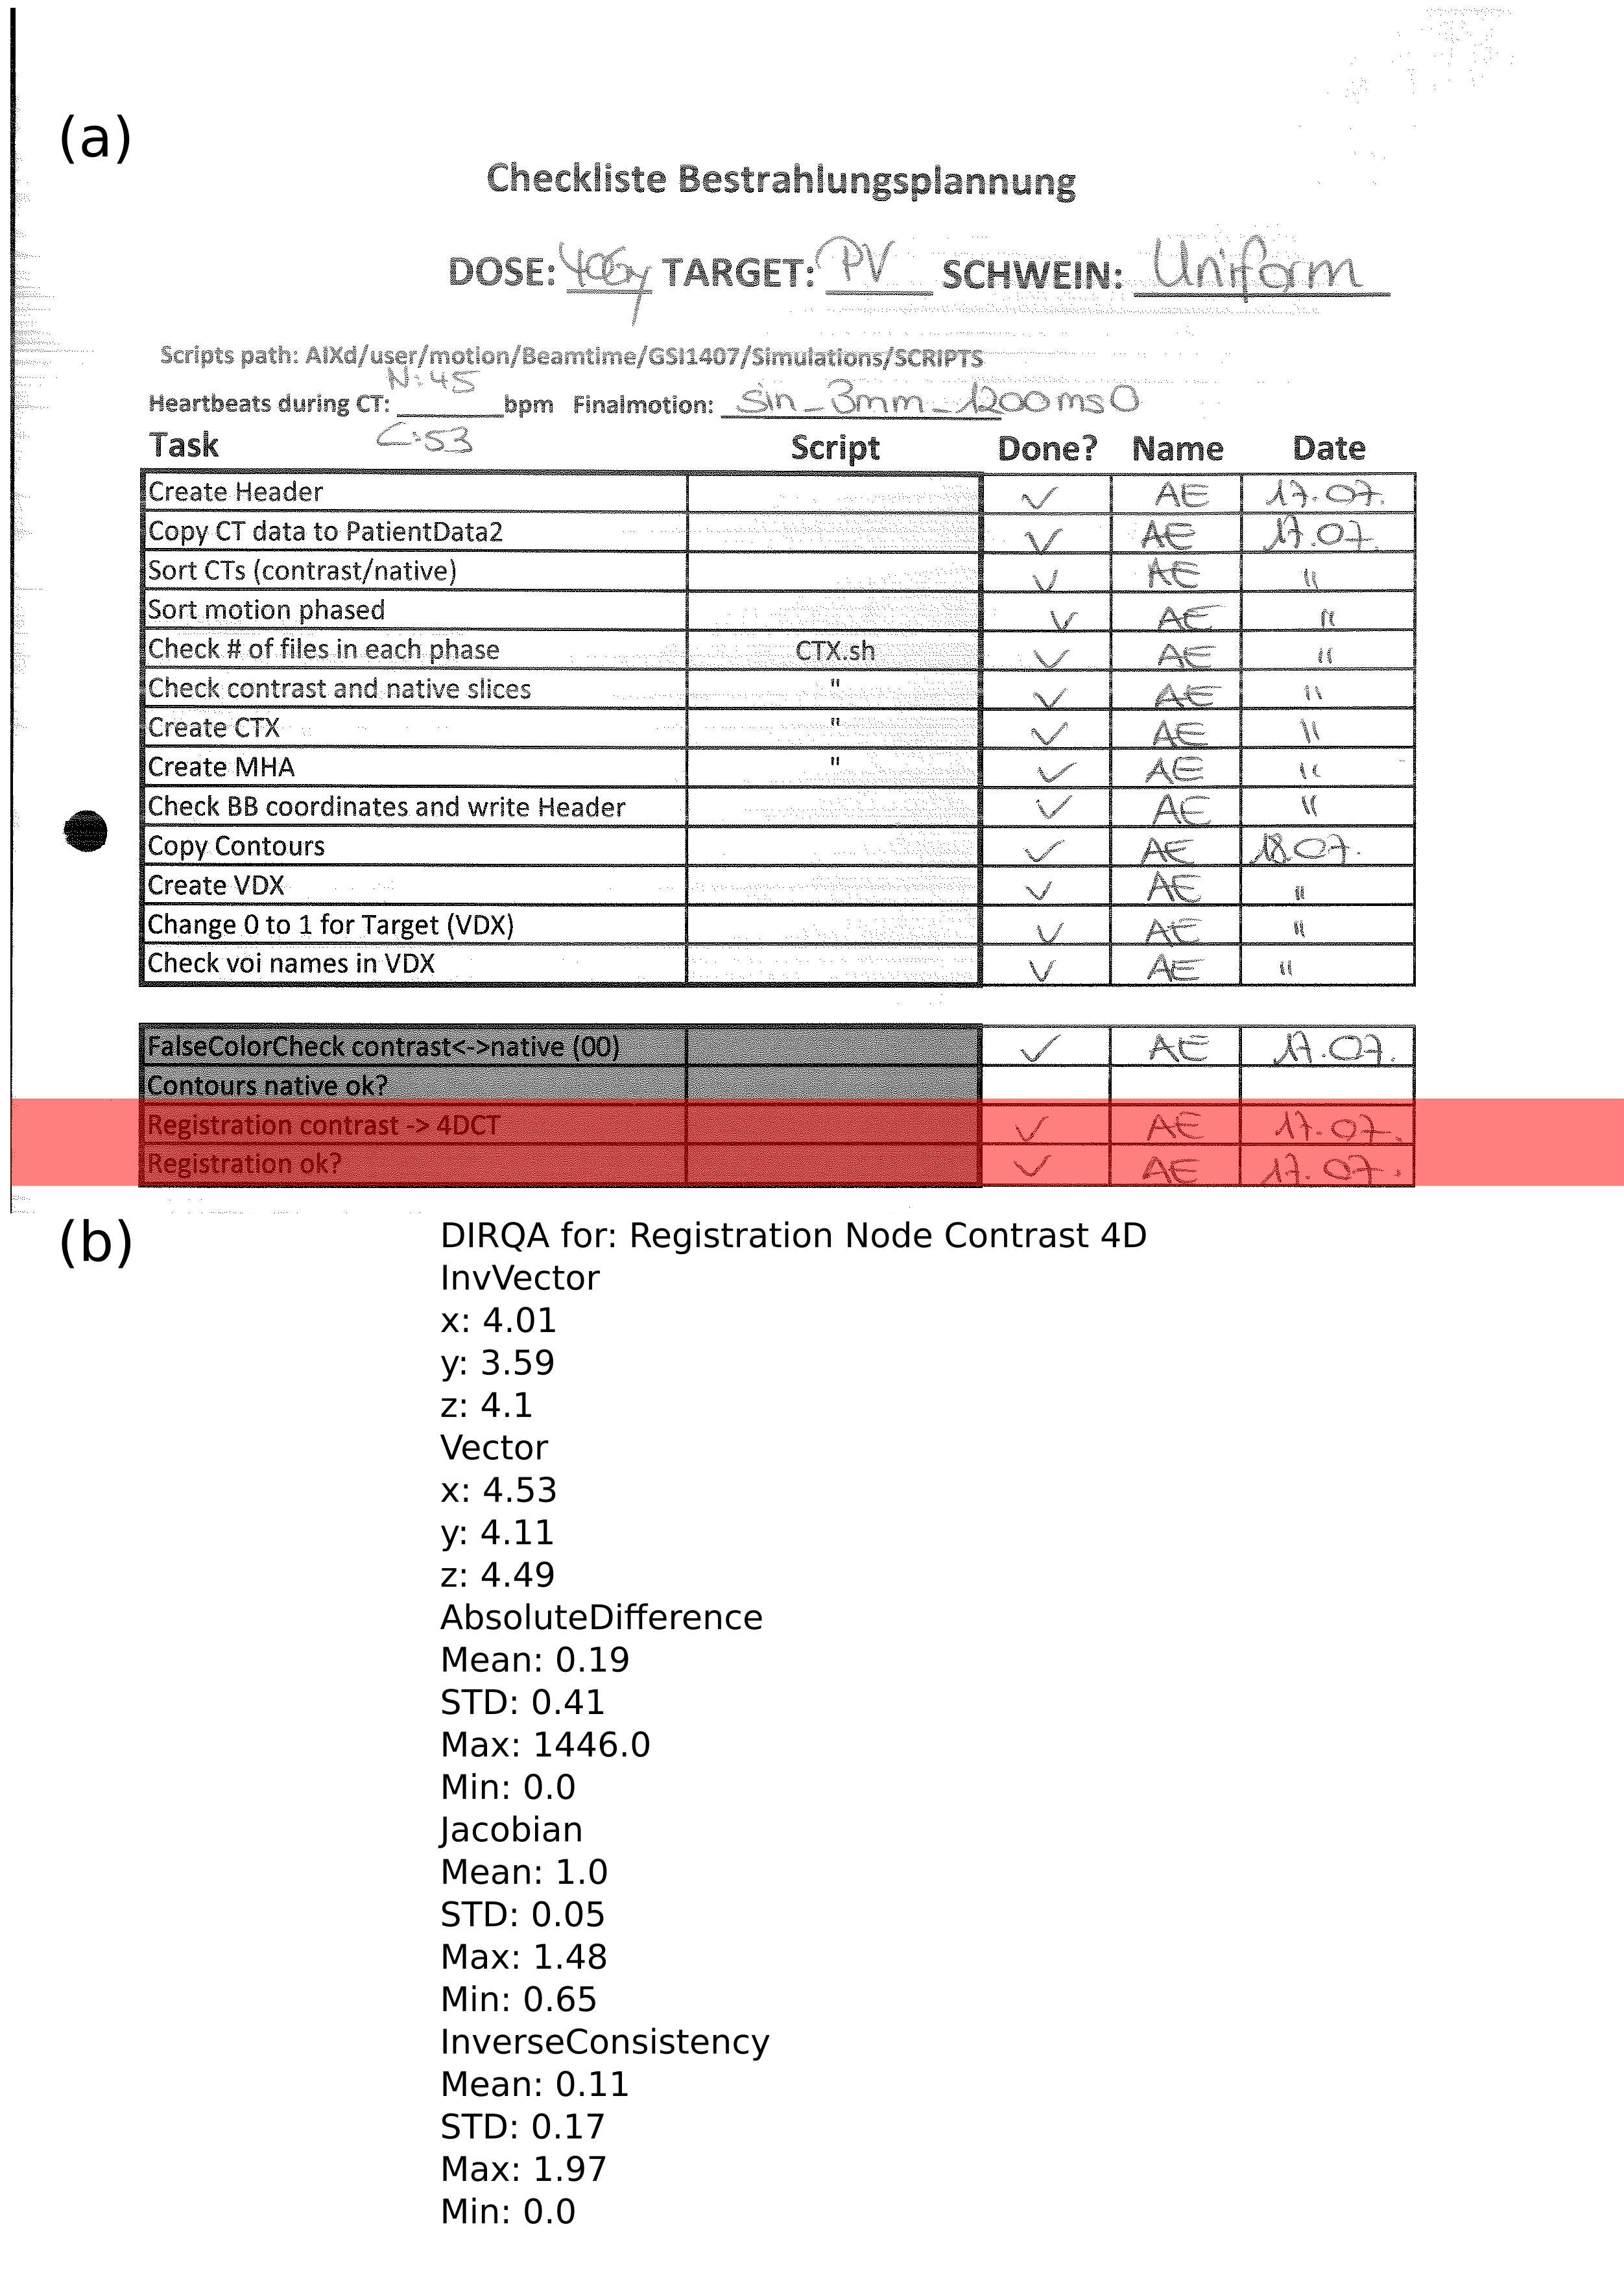
\includegraphics[width=0.9\textwidth]{./Images/checkList.png}
		\caption{(a) Part of the checklist for quality assurance during pig irradiation. DIR and DIRQA is highlited in red and consisted of two steps. First DIR was made on 4DCT-cardiac and afterwards DIRQA was made on
		DIR on phase 50\%. End result was presented as text shown in (b).}
		\label{checkList}
	\end{center}
\end{figure}
\newpage

\subsubsection{Results}


All DIRs were successful and during experiment all DIRQA checks were positive. An example of DIR is shown in Fig.~\ref{exampleReg_pigs}. A vector field analysis is shown in Table~\ref{tab:vectordata_pig}. No statistical difference was
observed between true and inverse vector field. However, significant diference was observed between vector field magnitudes of PM and noPM. Contributions to vector field magnitudes from three axis were equal. 


\begin{table}[H]
  \centering
%   \footnotesize
  \caption{Data for vector magintudes. Values are presented as average (range).}
  \begin{tabular}{c|c|c|c|c}
	    & \multicolumn{2}{|c|}{PM} & \multicolumn{2}{|c|}{noPM} \\
  
            & True vector field   & Inverse vector field   & True vector field  & Inverse vector field \\
       \hline
	Mean & 0.08 (0.03 - 0.16) & 0.08 (0.03 - 0.14) & 0.07 (0.0 - 0.18)  & 0.06 (0.0 - 0.17) \\ 
	STD  & 0.4 (0.09 - 0.78)  & 0.36 (0.08 - 0.68) & 0.3 (0.05 - 0.77)  & 0.28 (0.04 - 0.71) \\ 
	Max  & 8.24 (1.6 - 17.33) & 7.98 (0.7 - 17.76) & 5.9 (0.97 - 15.91) & 5.38 (1.08 - 12.42) \\ 
    \hline\hline
  \end{tabular}
  \label{tab:vectordata_pig}
\end{table}

\begin{figure}[H]
	\begin{center}		
		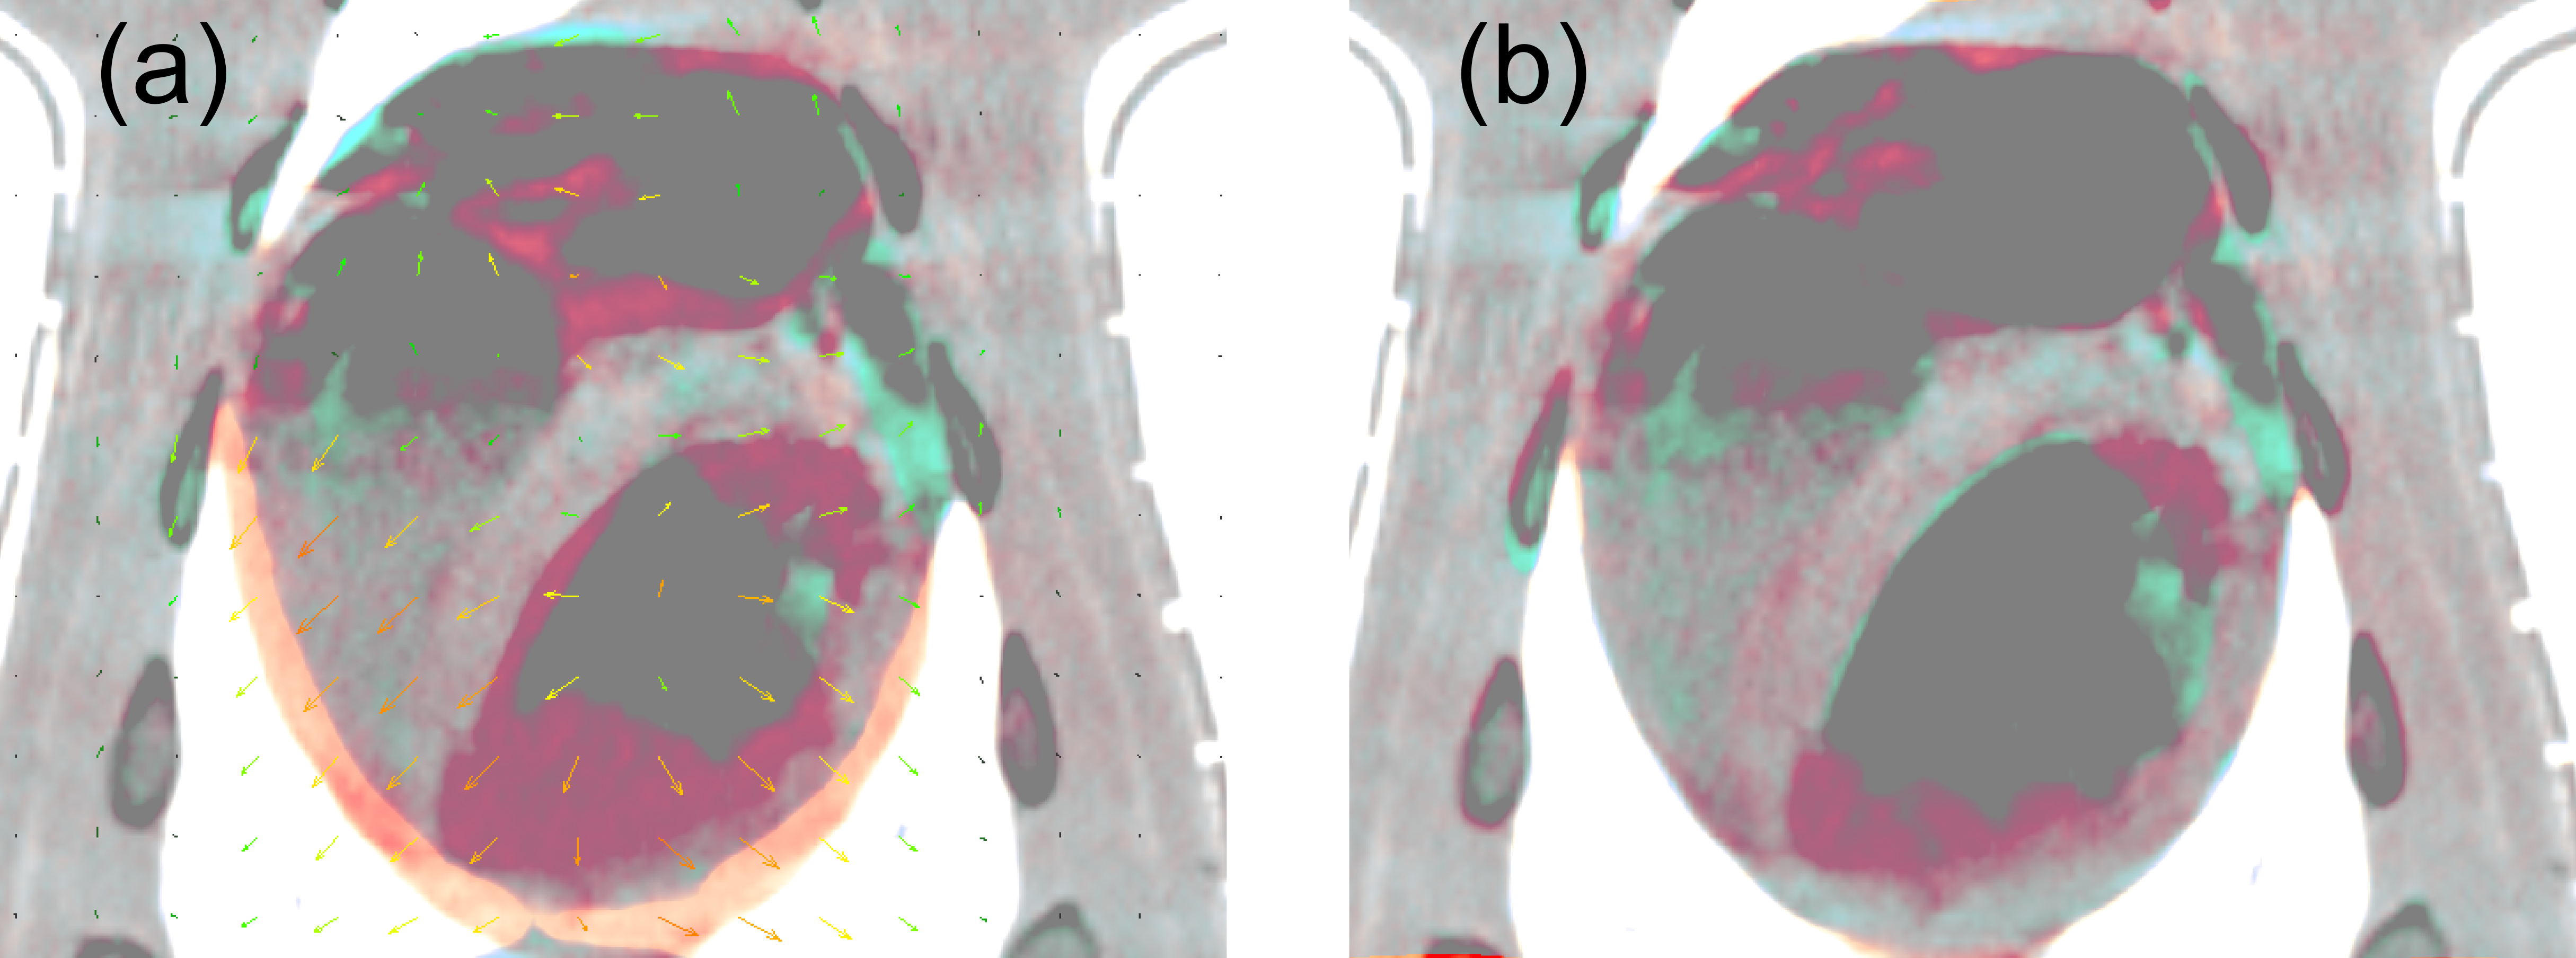
\includegraphics[width=0.9\textwidth]{./Images/exampleReg_pigs.png}
		\caption{False color overlay of two phases before (a) and after (b) DIR. Vector field is displayed on image (a) as arrows.}
		\label{exampleReg_pigs}
	\end{center}
\end{figure}

Dependence of true and inverse absolute difference on default absolute difference with a linear fit is shown in Fig.~\ref{absDiff_pigs}. Default absolute difference distribution accross 9 phases can be seen in inset in Fig.~\ref{absDiff_pigs}.

Distribuition of Jacobian and ICE results are shown in Fig. \ref{jacobian_data_pigs} and \ref{ice_pigs}. Maximum values of true and inverse maximum and minimum Jacobian and ICE were tested 
against maximum vector magnitudes and fitted with linear function. Results are plotted in Fig.~\ref{maxvf_pigs}.
Additionally, dependence of maximum true Jacobian on minimum inverse Jacobian was tested and results are display in Fig~\ref{calcJac_pigs}.

All linear fits in Fig.~\ref{absDiff_pigs}, ~\ref{calcJac_pigs} and ~\ref{maxvf_pigs} were statistically significant (p < 0.05).

\begin{figure}[H]
	\begin{center}		
		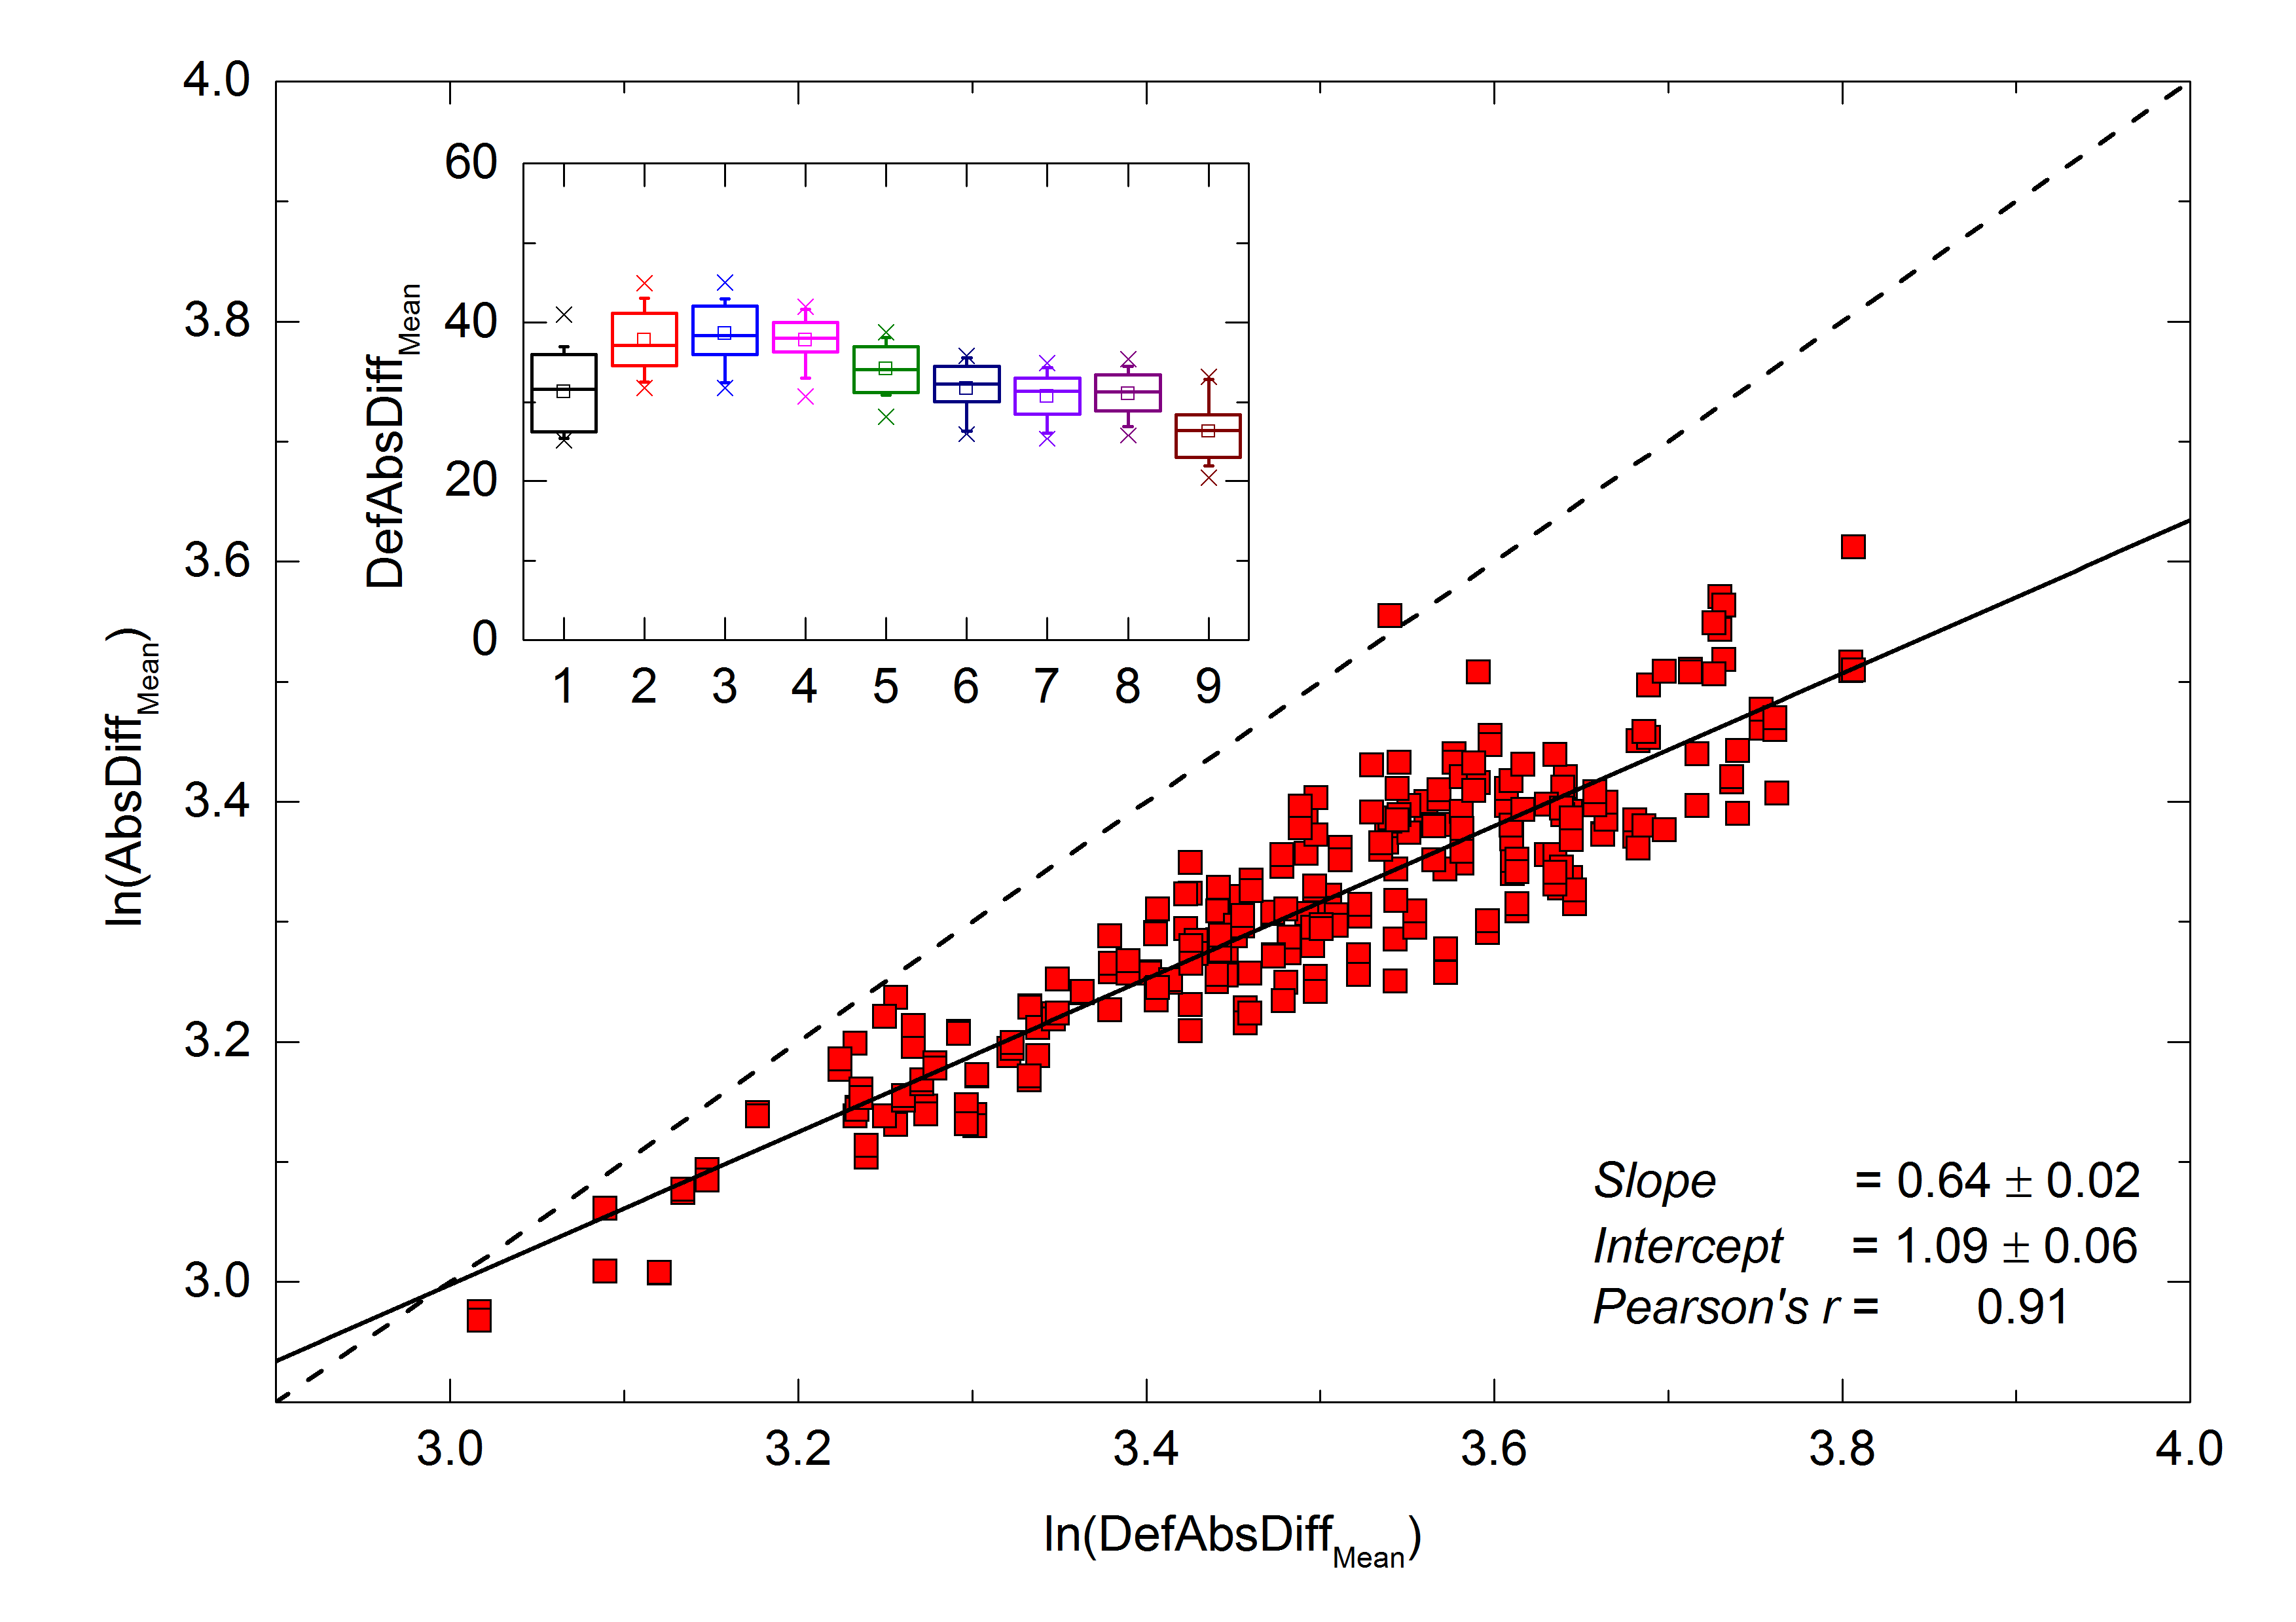
\includegraphics[width=0.9\textwidth]{./Images/AbsDiff_pigs.png}
		\caption{Natural logarithm of true and inverse absolute difference (AbsDiff) plotted against default absolute difference (DefAbsDiff). Solid line shows linear fit, with parameters
		writen in corner. Dashed line shows $y(x)=x$ plot. Inset shows box plots of mean distribution of default absolute difference across nine 4DCT phases. Boxes represent 25-75\%, whiskers 10-90\%
		of data, median is shown with solid line, mean with square and outliers with crosses.}
		\label{absDiff_pigs}
	\end{center}
\end{figure}


\newpage

\begin{figure}[H]
	\begin{center}		
		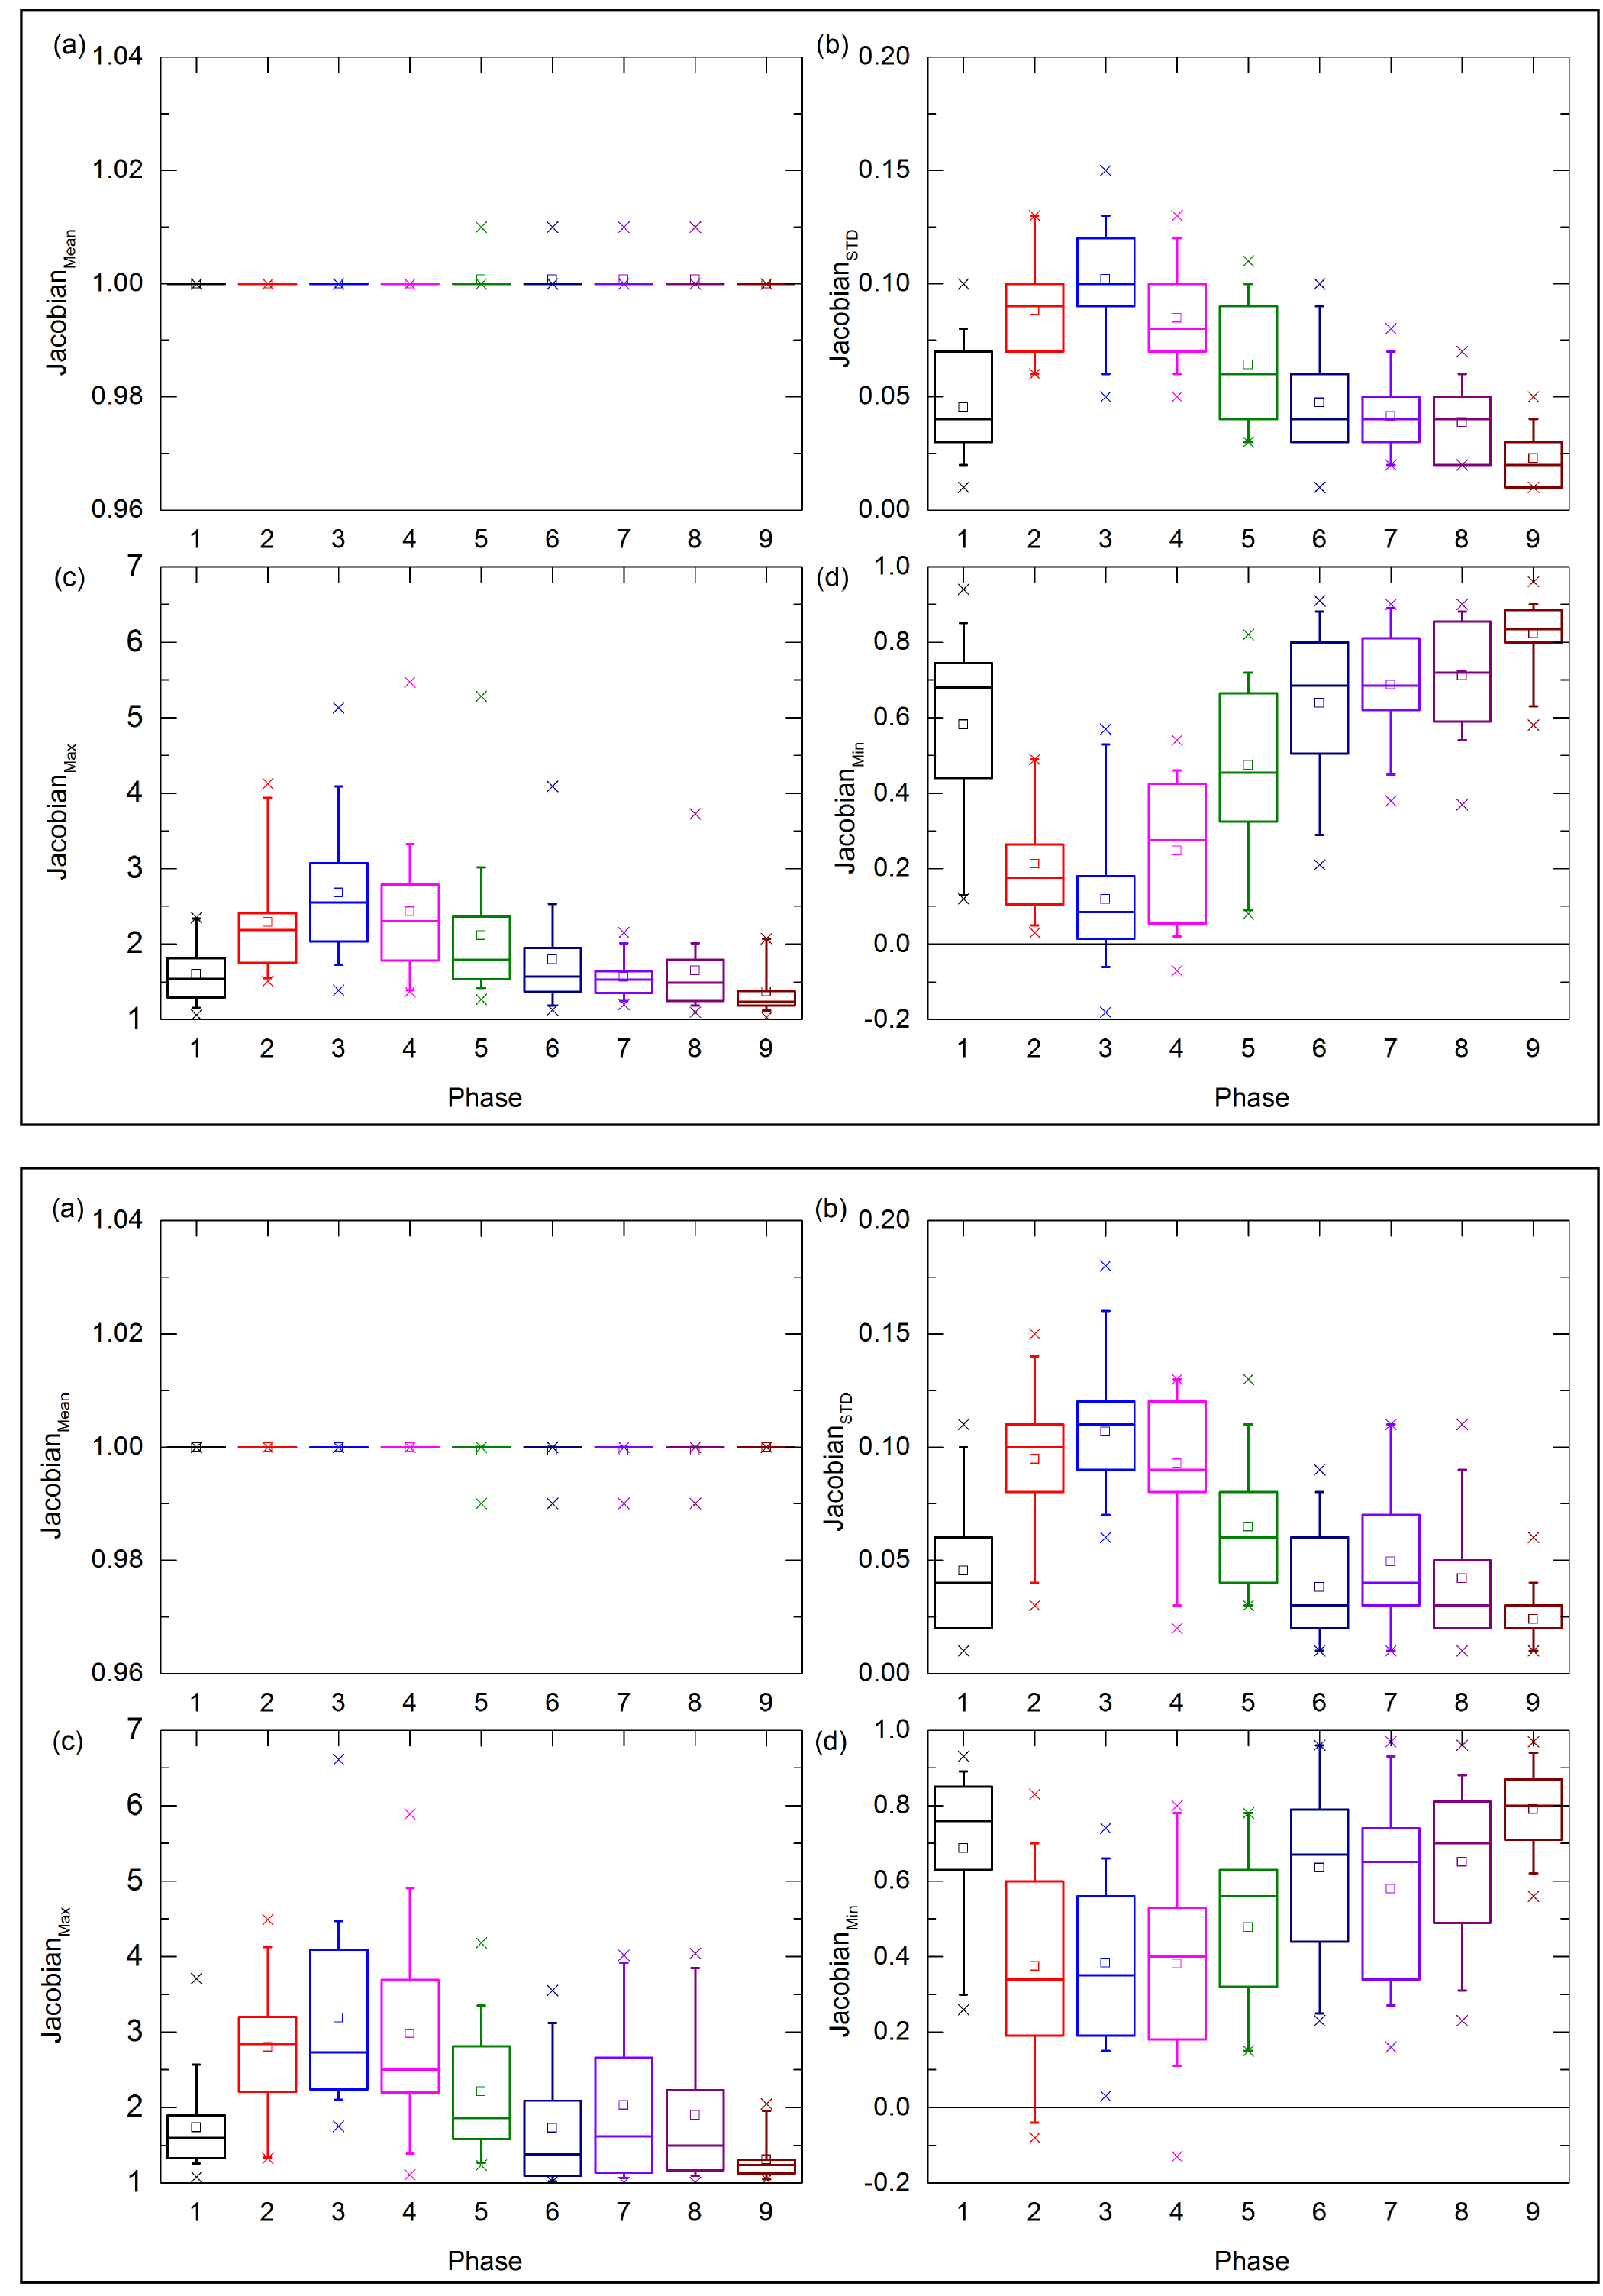
\includegraphics[width=0.75\textwidth]{./Images/Jacobian_data_pigs.png}
		\caption{Data for Jacobian of vector fields (top) and inverse vector fields (bottom) for 9 4DCT phases (reference phase 0 is excluded) for 23 lung cancer patients. Mean, STD, maximum and minimum are represented as (a), (b), (c) and (d), respectively.
		Boxes represent 25-75\%, whiskers 10-90\% of data, median is shown with solid line, mean with square and outliers with crosses.}
		\label{jacobian_data_pigs}
	\end{center}
\end{figure}

\newpage

\begin{figure}[H]
	\begin{center}		
		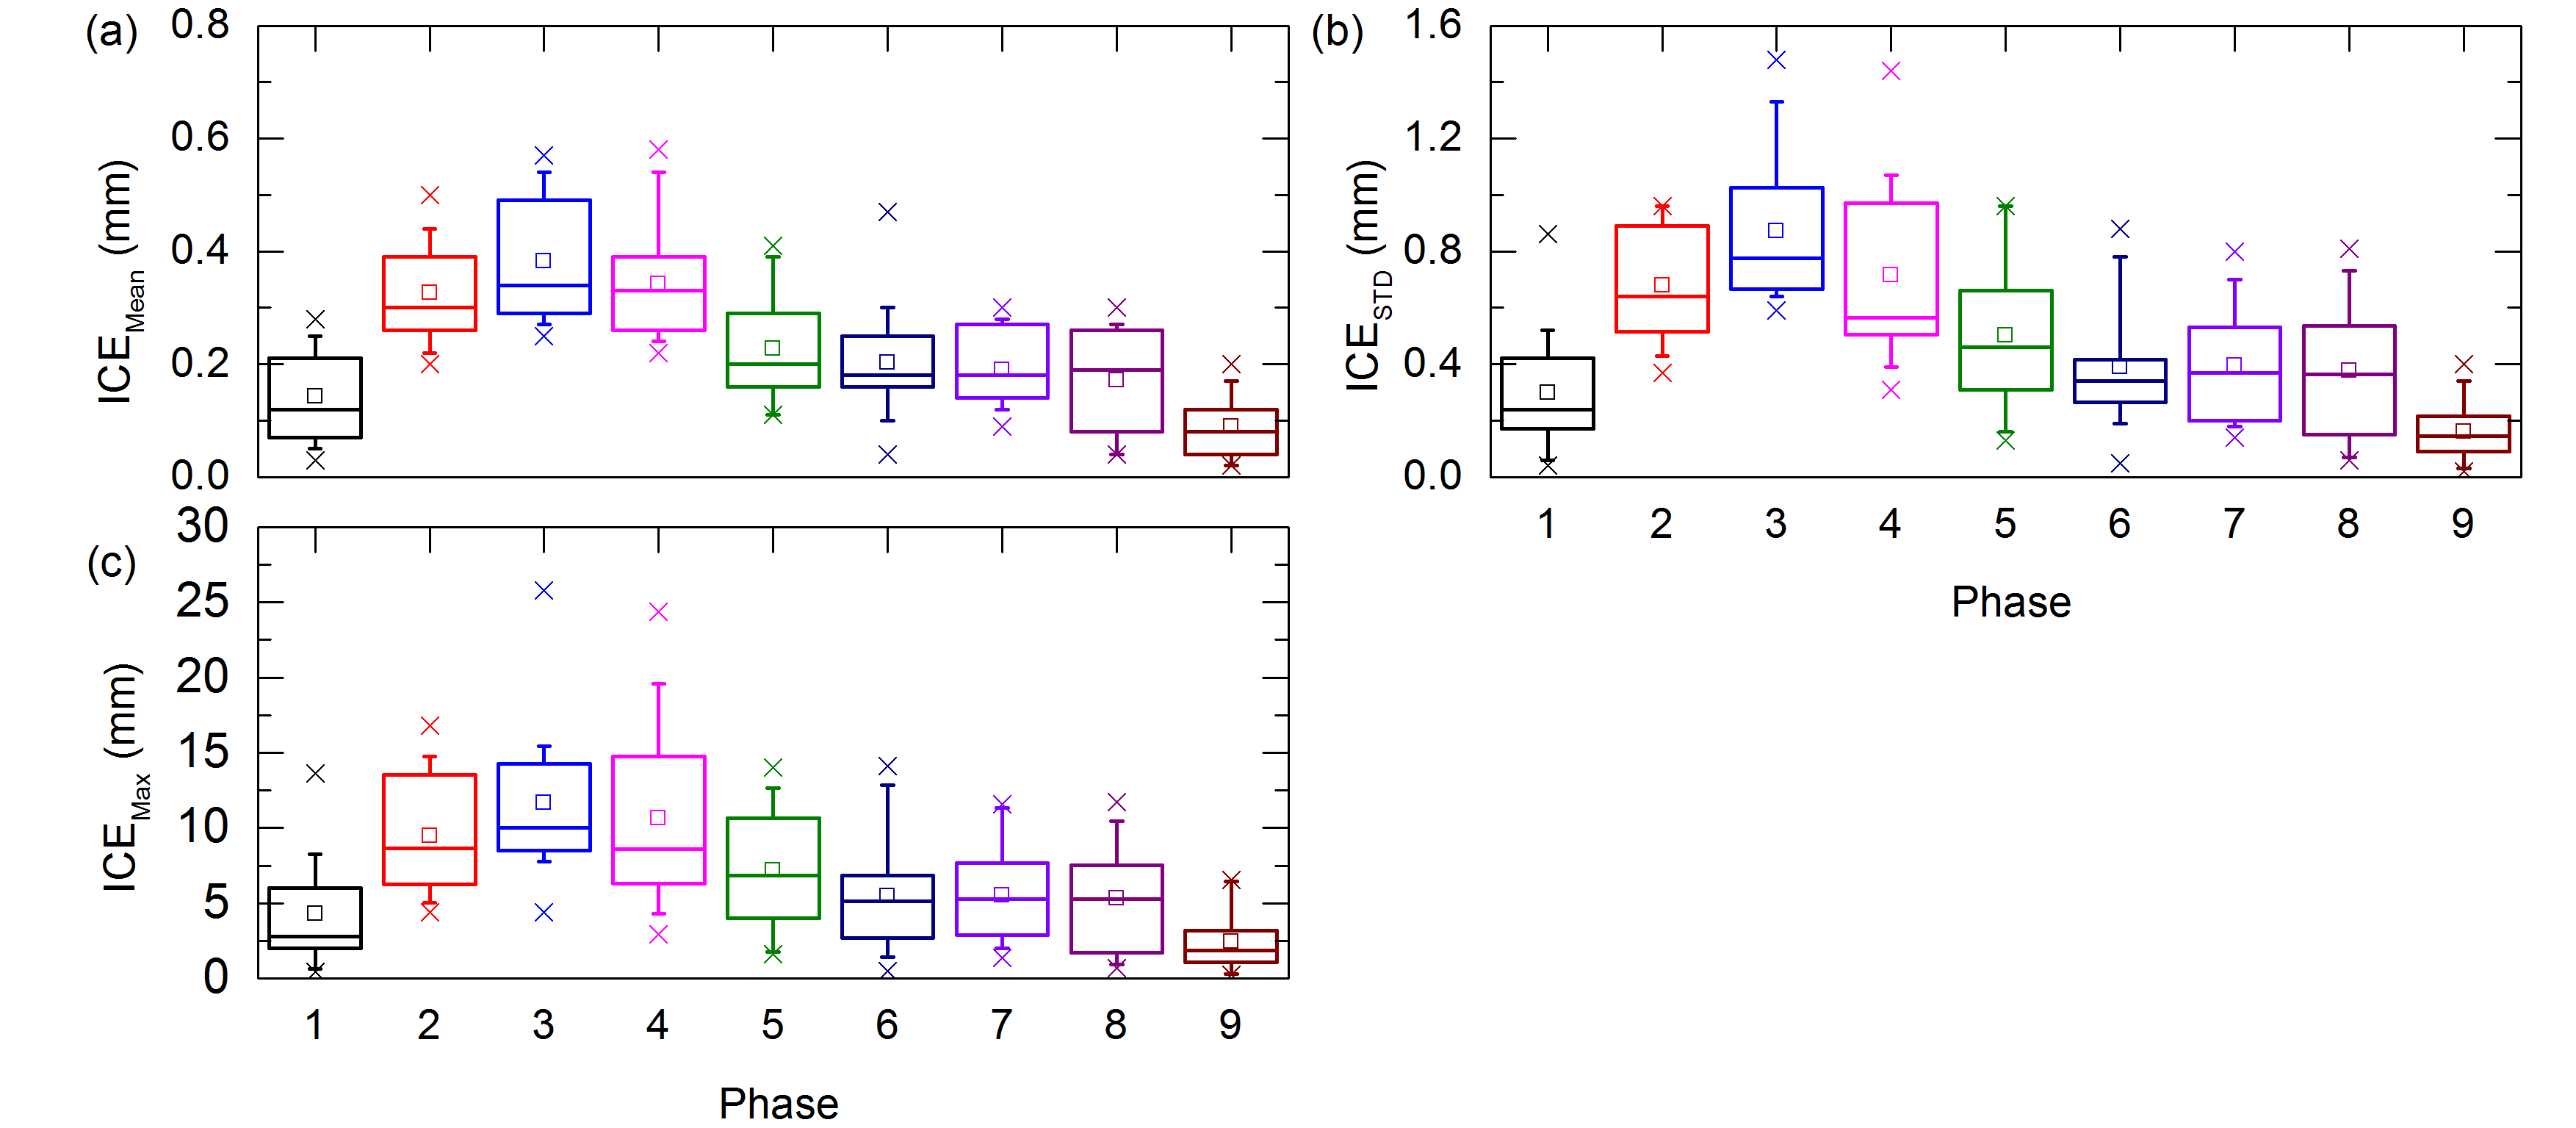
\includegraphics[width=0.9\textwidth]{./Images/ICE_pigs.png}
		\caption{Data for ICE for 9 4DCT phases (reference phase 0 is excluded) for 23 lung cancer patients. Mean, STD, maximum are represented as (a), (b) and (c), respectively. ICE Minimum is 0 throughout all phases and patients.
		Boxes represent 25-75\%, whiskers 10-90\% of data, median is shown with solid line, mean with square and outliers with crosses.}
		\label{ice_pigs}
	\end{center}
\end{figure}

\begin{figure}[H]
	\begin{center}		
		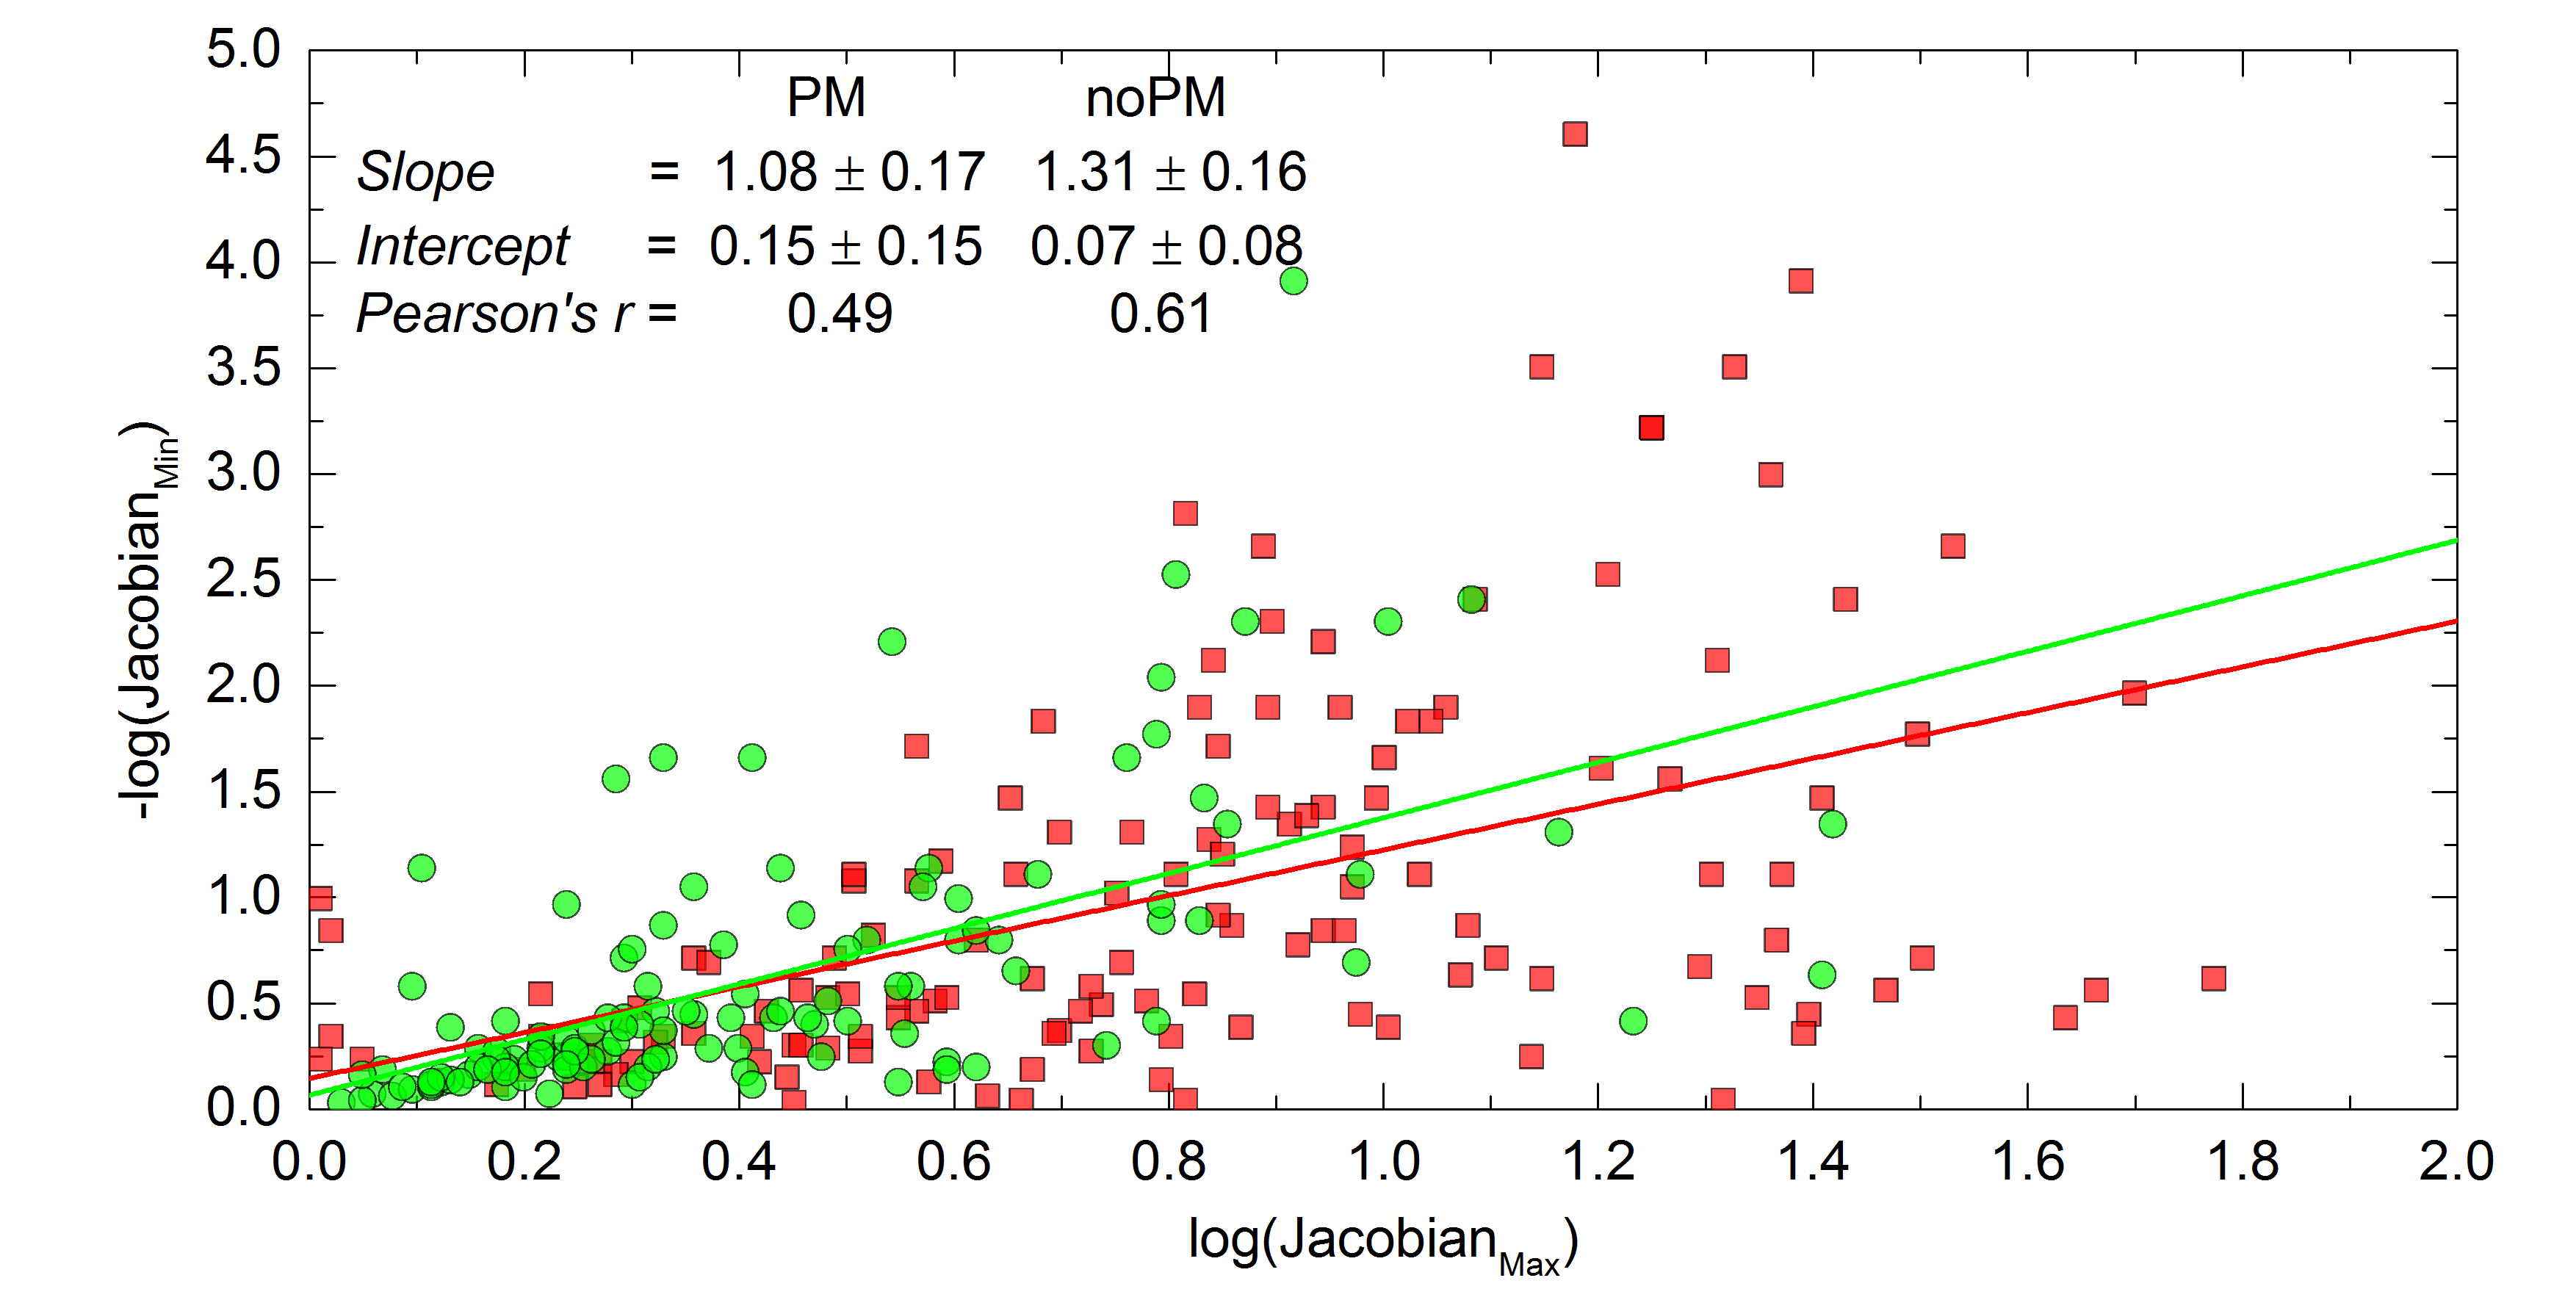
\includegraphics[width=0.9\textwidth]{./Images/JacSum2.png}
		\caption{(a) Plot of negative natural logarithm of minimum Jacobian versus maximum Jacobian. Linear fit is displayed with solid line and it's parameters are given in the corner.}
		\label{calcJac_pigs}
	\end{center}
\end{figure}

\begin{figure}[H]
	\begin{center}		
		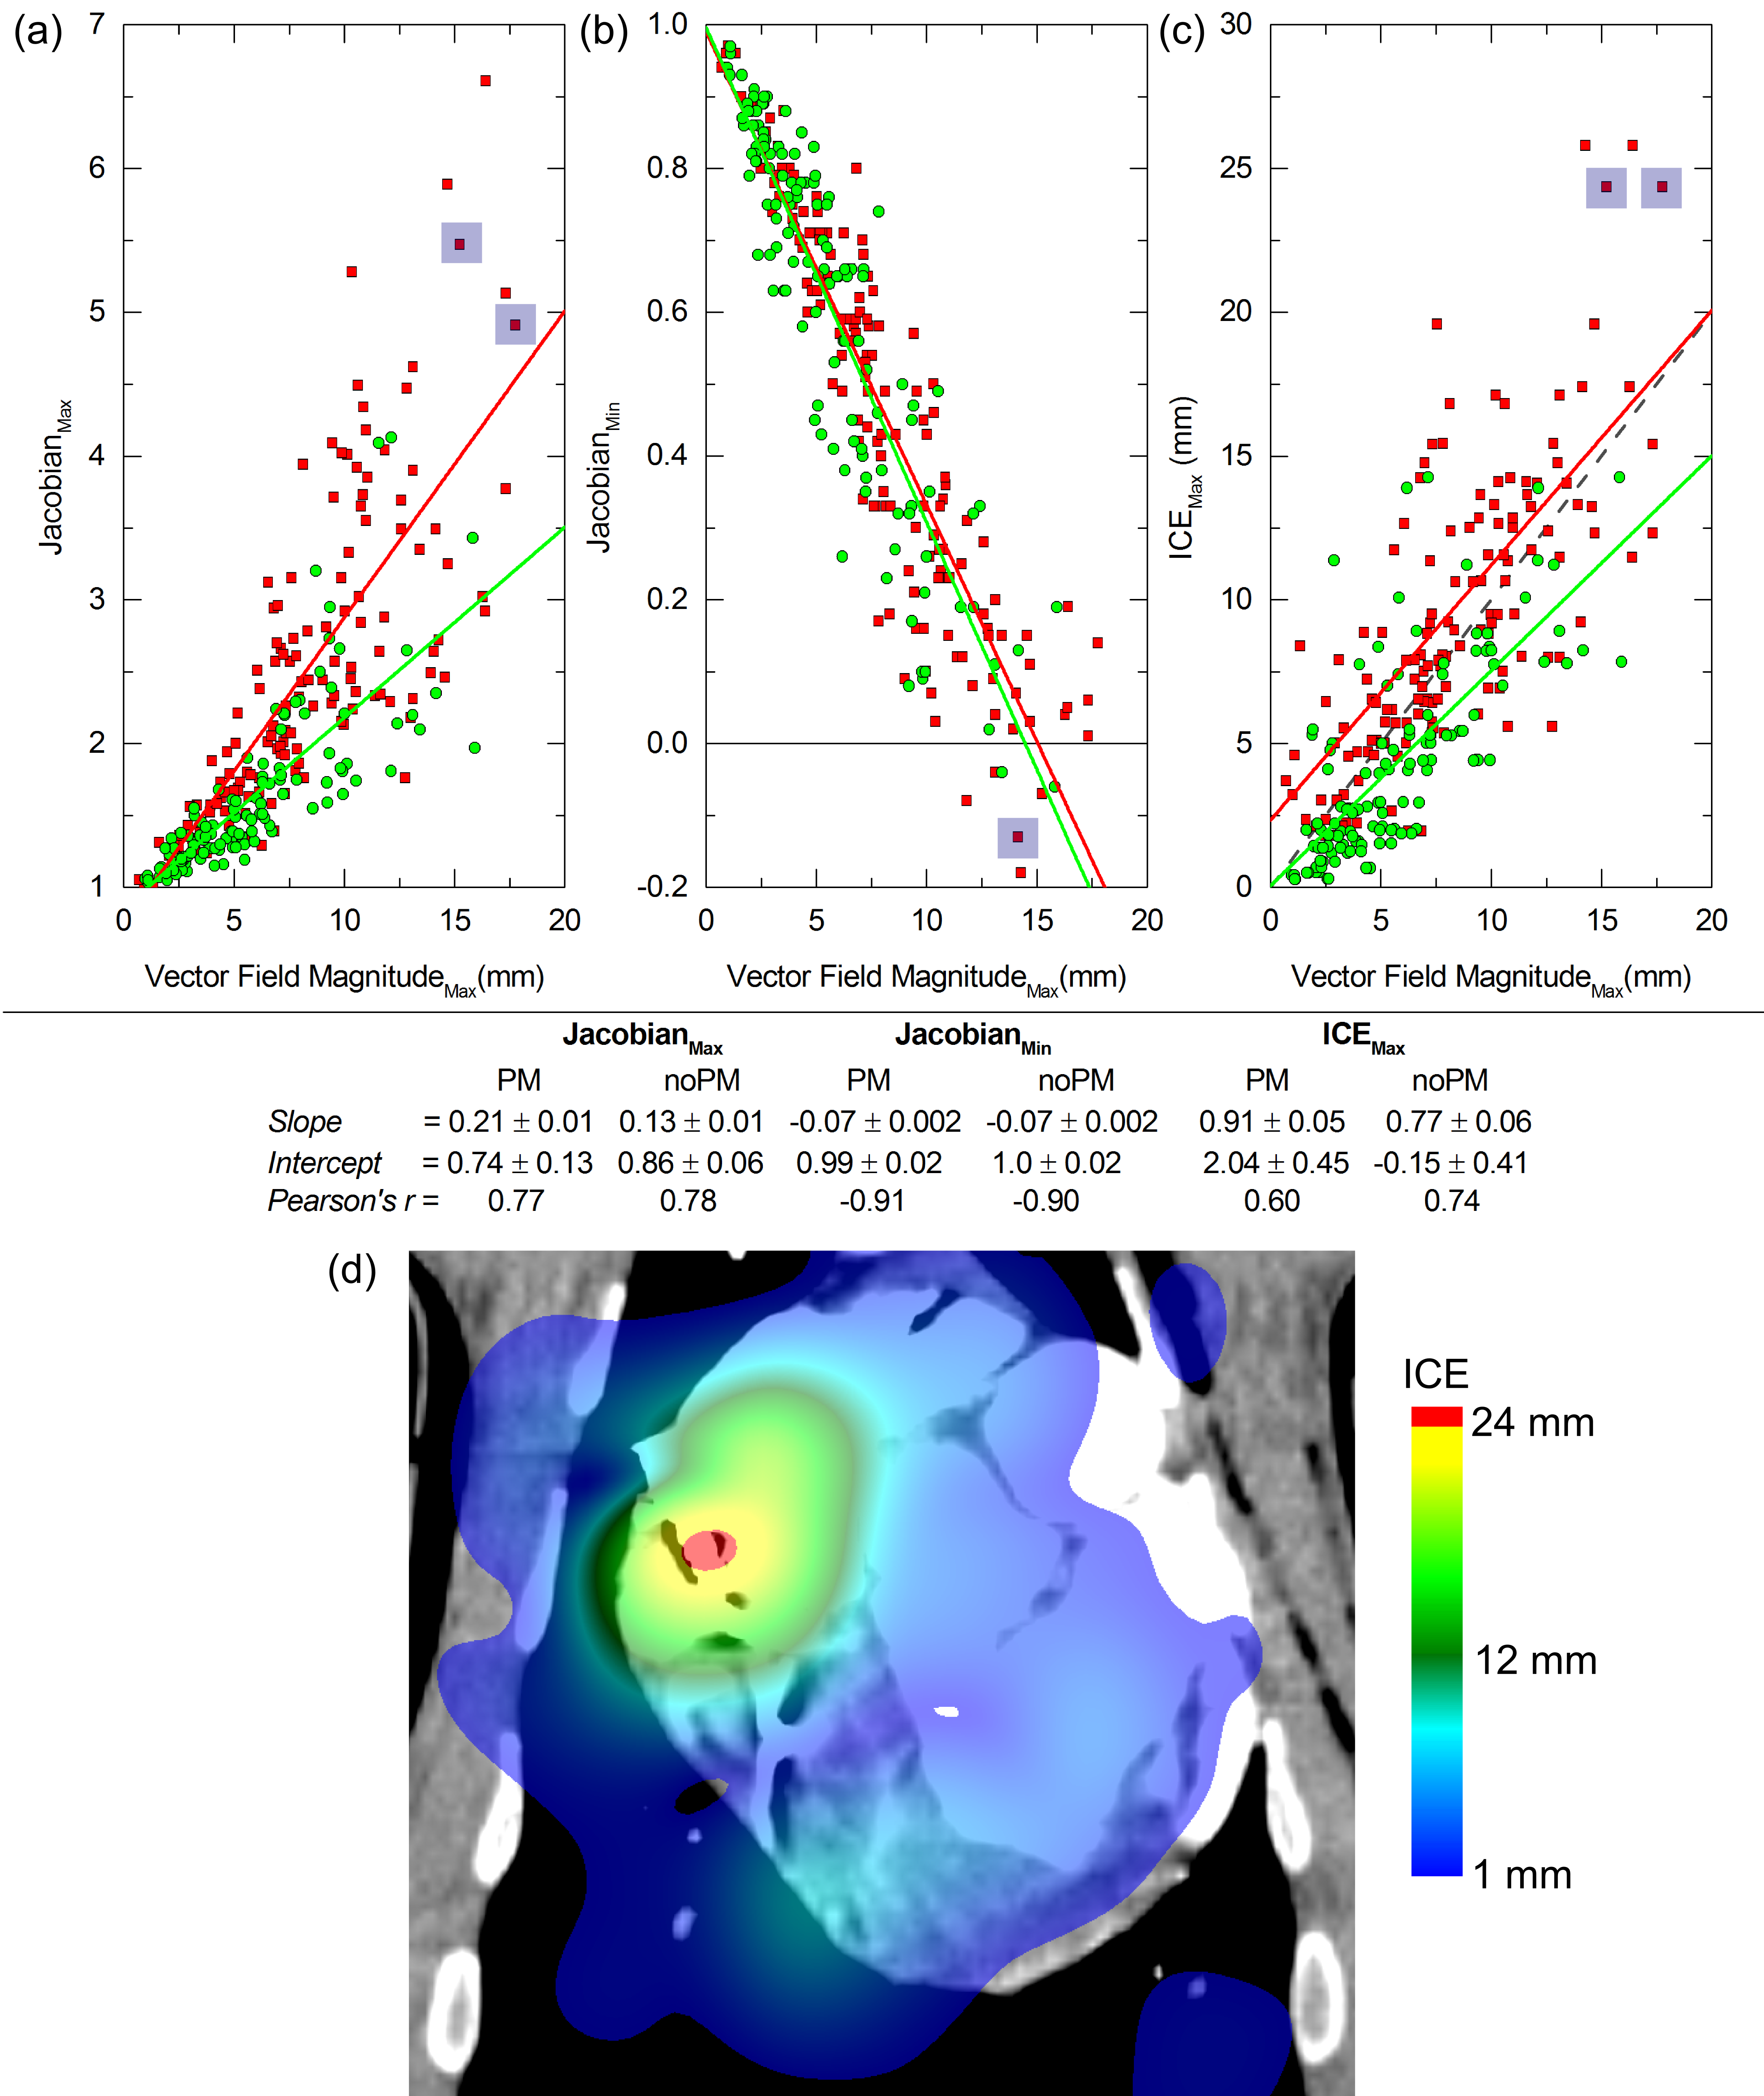
\includegraphics[width=0.9\textwidth]{./Images/MaxVfdata_pigs.png}
		\caption{Values of maximum Jacobian (a), minimum jacobian (b) and ICE (c) plotted against maximum vector magnitudes. Linear fit is displayed with solid line and parameters are written below the plots. Dashed line in (c) shows $y(x)= x$ plot. Values from patient on image (d) are highlighted with blue squares in (a)-(c).
			ICE is displayed on (d) using color table as displayed in legend.}
		\label{maxvf_pigs}
	\end{center}
\end{figure}


\subsubsection{Discussion}

Mean vector field magnitudes were small (approx. 0.1 mm), since pigs were in a breath-hold position and the only motion was the beating of the heart. 
Despite the small mean vector magnitude it was still enough to observe statistical difference between the PM and noPM.
Consequently, the difference between the two groups is consistent throughout the DIRQA.

The DIR did well in terms of lowering the absolute difference metric. There was a strong correlation between default versus true and inverse absolute difference. The shape of default absolute difference
distribution persist then in other DIRQA check as well.

A good result in absolute difference does not necessary mean a good DIR, as can be seen from Jacobian and ICE checks. The mean Jacobian and ICE were 1 and 0, respectively, since the
vector fields were small on average. However there were large deviations present in Jacobian and ICE. Most notably, there were a few cases of negative minimum Jacobian which would suggest 
organ folding. Since organ folding did not occur during a heart beat, negative minimum Jacobian points to inconsistencies in DIR. The inconsistencies in DIR can be also seen on Fig~\ref{calcJac_pigs},
with a poor correlation between minimum inverse and maximum true Jacobian. The correlation is better for noPM, however there are still cases that deviate from linear fit.

The large deviations in Jacobian and ICE can in part be explained with large maximum vector field values, as shown in Fig.~\ref{maxvf_pigs}. All linear fits have good correlation, with no
difference between PM and noPM in the quality of the fits. The actual linear fit parameters, however, further show the inconsistencies in DIR. The clearest example of inconsistencies in
DIR is with linear fit from maximum ICE PM, which lies above $y(x)=x$ function. This basicaly means that tere were points further away from starting point after true and inverse transformation, 
then by just after true transformation. The linear fit for maximum ICE showed better results in this terms, since it layed below $y(x)=x$ function.


% \subsection{Mid-Position patient example}


\section{Summary and Discussion}

Tools to preform DIR and DIRQA were presented in this chapter. Different modules were written for an open-source software Slicer, that can handle large DIR problems, such as registering whole 4DCT. In addition to DIR the modules can also make DIRQA on the same set as DIR was made with several different
checks. The main objective of this work was to provide systematic approach to DIR and to give parameters on DIRQA that can estimate the quality of DIR. A first analysis of DIRQA checks was done on a large DIR database - 684 DIR were checked in total.

Most of the work was based on Slicer, which is well-established software in medical research. To date, there are more than 500 publications that have used Slicer in their research \cite{SlicerCitation}, with topic ranging from 
teaching \cite{Pujol2016}, disease staging \cite{Liu2016, Liu2015}, motion tracking \cite{Behringer2015} to image reconstruction \cite{Meyer2015}, image registration \cite{Li2015, Fedorov2015, Li2015}
and others. Slicer offers a lot of different functionalities and is especially good for research, since it can be modified to specific needs. However, it is important to stress that Slicer 
is not a medical application and can be used only for research. Additionally, Slicer can sometimes be unstable with unexpected crashes. It is constantely under development and more and more errors
are fix with each new release. New releases also bring new functionalities, but there can be problems with backtrack compability. Even though there are some disadvantages to using Slicer, it's advantages
defenetily outweigh them and make Slicer a useful tool, as was showed in this chapter.

Results shown in this chapter were obtained with DIR made by B-Spline algorithm. Several other algorithms exist, demons most commonly used alongside B-Spline \cite{Thirion1998}. Varadhan et al. made comparison
between B-Spline and demons DIR for lung case \cite{Varadhan2013} and showed that B-Spline is superior to demons, especially if there is difference in contrast between images. They used mutual information
metric, to account for differences in contrast. Images used in this chapter were either all without (lung case) or all with (pig case) contrast agent, therefore there was no difference in contrast
between images. Mutual information metric was tested as well for DIR, however the results were much worse than mean square error metric.

The evaluation of DIR was made by DIRQA module. The main advantage of the DIRQA module is that all different tecniques are gathered in a single place and can be used on a specific case. The ease of use is also essential, for DIRQA to find it's way into clinical workflow.
A test of using DIRQA in potential clinical workflow was done at GSI during pig experiment, where different users had to use both DIR and DIRQA modules. The experiment was also under time pressure, since there is
a scheduled beam time and it cannot be shifted. There were already prepositions for frameworks for DIRQA in clinical workflow \cite{Varadhan2013}, however none were actually tested.

The techniques used in DIRQA can be divided into visible (false color, checkerboard) and quantitative (absolute difference, Jacobian and ICE). While the quantitative can be used to pinpoint errors in DIR, the visible can be used to actually see the error and how does it affect the
end result, as shown in Fig.~\ref{calcJac_lung})c. All three quantitative checks have been used in literature as a possible DIRQA \cite{Varadhan2013, Leow2007, Christensen2001, Bender2009}. They all share the same flaw, however, that they are a necessary condition for a successful
DIR but not sufficient. One common DIRQA check in literature that our module is currently missing, is comparison of anatomical correspondence - comparison between reference, moving and warped contours. Ideally warped and reference contour should be the same. Two metrics are used in contour comparison -
dice similarity coefficient \cite{Varadhan2013} and Hausdorff distance \cite{Huttenlocher1993}. Slicer already has functionalities for both contour comparison checks, so they could be used. The biggest disadvantage of anatomical correspondence check is that contour delineation is required in both, reference and moving phase, which is almost never done by physicians, since it takes too much time. Lack of contour in both, reference and moving phase, was also the reason the anatomical correspondence check was not used.

Studies on DIRQA so far have focused on a small number of DIR cases, weather it is phantom \cite{Mutic2001,Moore2004} or patient studies \cite{Wu2008, Varadhan2013}. With small number of DIR it is possible to thourgouly examine each DIR, so that DIRQA can be explained. In this chapter a different approach was
used. Rather than examining each DIR individually, a large dataset was analyzed and common traits for DIR were found.





\bibliographystyle{apalike}
\bibliography{../ref.bib}{}
% \bibliographystyle{plain}

\end{document}
